\documentclass[a4paper,12pt,oneside,openany]{book}

% ============================================================================
% DOCUMENTAÇÃO DO PROJETO FINAL - ENGENHARIA DE SOFTWARE II
% UNESP - Faculdade de Ciências - Departamento de Computação
% Sistema Unespão
% ============================================================================

\usepackage[T1]{fontenc}
\usepackage[utf8]{inputenc}
\usepackage{lmodern}
\usepackage[brazil]{babel}
\usepackage{graphicx}
\usepackage{booktabs}
\usepackage{tabularx}
\usepackage{array}
\usepackage{enumitem}
\usepackage{hyperref}
\usepackage{natbib}
\usepackage{fancyhdr}
\usepackage[top=2cm,bottom=2cm,left=2cm,right=2cm]{geometry}
\usepackage{xcolor}
\usepackage{listings}
\usepackage{microtype}
\usepackage[htt]{hyphenat}
\usepackage{float}

% Evita que palavras longas (identificadores de código em \texttt) estourem
% a margem: permite quebra dentro delas quando não há outra opção, e dá mais
% folga ao algoritmo de justificação antes de forçar uma caixa "overfull".
\tolerance=1000
\emergencystretch=3em
\hyphenpenalty=300
\exhyphenpenalty=300

\hypersetup{
    hidelinks,
    pdftitle={Documentação do Projeto de Software},
    pdfauthor={Equipe do projeto}
}

\urlstyle{same}

% ----------------------------------------------------------------------------
% Configuração de listagens de código (C#)
% ----------------------------------------------------------------------------
\lstdefinelanguage{csharp}{
    morekeywords={public,private,protected,internal,class,readonly,static,void,var,new,return,using,namespace,if,else,throw,async,await,true,false,null},
    sensitive=true,
    morecomment=[l]{//},
    morestring=[b]"
}
\lstset{
    basicstyle=\ttfamily\scriptsize,
    numbers=left,
    numberstyle=\tiny\color{gray},
    breaklines=true,
    frame=single,
    backgroundcolor=\color{gray!5},
    commentstyle=\color{gray!70!black},
    keywordstyle=\color{blue!60!black},
    stringstyle=\color{green!40!black},
    showstringspaces=false,
    tabsize=2,
    captionpos=b
}

% ----------------------------------------------------------------------------
% Exibição das orientações do template (desativada nesta versão de entrega)
% ----------------------------------------------------------------------------
\newif\iforientacoes
\orientacoesfalse

\newcommand{\orientacao}[1]{%
    \iforientacoes
        \begin{quote}
        \small\itshape\textbf{Orientação:} #1
        \end{quote}
    \fi
}

% ----------------------------------------------------------------------------
% Cabeçalho e rodapé
% ----------------------------------------------------------------------------
\renewcommand{\headrulewidth}{0pt}
\fancyhf{}

% ----------------------------------------------------------------------------
% Informações do trabalho
% ----------------------------------------------------------------------------
\newcommand{\school}{Universidade Estadual Paulista ``Júlio de Mesquita Filho'' (UNESP)\\
Faculdade de Ciências -- Bauru\\
Departamento de Computação}
\newcommand{\discipline}{Engenharia de Software II}
\newcommand{\projtitle}{Sistema Unespão}
\newcommand{\projsubtitle}{Plataforma de Pedidos Personalizados para Padarias}
\newcommand{\semester}{2026}

\graphicspath{{images/}}

\title{Documentação do Projeto de Software}
\author{Equipe do projeto}

\begin{document}

% ============================================================================
% CAPA
% ============================================================================
\thispagestyle{empty}
\begin{titlepage}
	\centering

	\vspace*{-12mm}
	
\includegraphics[width=75mm]{AV01A.jpg}\\[8mm]

	{\large\textbf{\school}}

	\vfill

	{\huge\textbf{\projtitle}}\\[5mm]
	{\Large\projsubtitle}

	\vfill

	{\Large\textbf{\discipline}}\\[14mm]

	David Almeida Saragó -- RA: 241021081\\[2mm]
	Guilherme Molina Trindade -- RA: 241023998\\[2mm]
	Lucas Costa Oliveira -- RA: 241023076\\[2mm]
	Thiago Mitsuo da Silva Nomura -- RA: 241023319

	\vfill

	{\large Bauru -- SP\\\semester}
\end{titlepage}

\tableofcontents
\thispagestyle{empty}

\clearpage
\pagestyle{fancy}
\cfoot{\thepage}
\setcounter{page}{1}

\iforientacoes
\chapter*{Como utilizar este modelo}
\addcontentsline{toc}{chapter}{Como utilizar este modelo}

Este documento é um roteiro para apoiar a documentação do projeto final.
Os textos marcados como \textit{Orientação} explicam o que se espera em
cada parte e podem ser ocultados alterando-se, no início do arquivo,
\verb|\orientacoestrue| para \verb|\orientacoesfalse|.

O documento deve registrar as principais decisões do projeto, e não apenas
reunir diagramas. Sempre que uma escolha relevante for apresentada, expliquem
brevemente a motivação e suas consequências. Diagramas, tabelas e protótipos
devem ser mencionados e explicados no texto.

Não é necessário documentar todas as classes, telas ou detalhes internos do
sistema. Em projetos maiores, priorizem os elementos mais relevantes,
complexos ou representativos.

\clearpage
\fi

% ============================================================================
\chapter{Introdução e Objetivos}
% ============================================================================

O Sistema Unespão é uma plataforma digital para a padaria Unespão que permite a clientes montarem e finalizarem pedidos de lanches personalizados, no estilo adotado por redes como Subway e Spoleto. Este capítulo situa o problema que o software resolve, delimita seu escopo, apresenta uma visão geral dos requisitos identificados a partir do domínio do negócio e estabelece os objetivos de qualidade que devem orientar as decisões de projeto detalhadas nos capítulos seguintes.

\section{Contexto do software}

A padaria Unespão opera sob um modelo de atendimento em que o cliente não escolhe apenas entre itens de cardápio fixos, mas monta o próprio lanche a partir de uma base (por exemplo, tipo de pão, massa de bolo ou base de salada) combinada com ingredientes adicionais (recheios, molhos, coberturas e acompanhamentos). Esse processo de personalização, hoje realizado sem suporte informatizado dedicado, sofre com a lentidão no atendimento, com a dificuldade de manter o controle de estoque dos insumos disponíveis e com a ausência de mecanismos que aproveitem o histórico de consumo do cliente para oferecer recomendações relevantes.

A finalidade do sistema, conforme definida pela equipe, é otimizar o processo de pedido e personalização de produtos, melhorar a experiência do cliente e aumentar a fidelização por meio de sugestões personalizadas de lanches. Para isso, o sistema passa a intermediar toda a jornada do cliente: da escolha da base e dos ingredientes até o registro do pedido, o pagamento da transação, a avaliação do prato consumido e o recebimento de sugestões baseadas em seu histórico.

Dois pontos dessa jornada aparecem com mais destaque na Visão Arquitetural (C4 Nível 1 e Nível 2) do que no relato inicial de Minimundo, e por isso merecem uma menção explícita aqui. O primeiro é o pagamento: o sistema se integra a um gateway de pagamento externo para processar as transações financeiras dos pedidos, e o \texttt{PedidoService} responde pelo ciclo do pedido desde a criação até a personalização dos itens e o processamento do pagamento. Do ponto de vista do cliente da padaria, um pedido só está de fato concluído depois de pago; por isso tratamos pagamento como parte natural do fluxo descrito neste capítulo, não como uma etapa à parte. O segundo ponto é a autenticação: o cliente se identifica junto à plataforma por meio de um serviço de autenticação externo (Google, via OAuth 2.0), o que permite ao sistema reconhecer um cliente recorrente, associar seu histórico de pedidos e, a partir daí, sustentar a geração de sugestões personalizadas.

O principal interessado direto no sistema é o cliente, que interage com a plataforma por meio de totens físicos instalados na loja ou de um aplicativo móvel, ambos servindo como canal de montagem, pagamento e envio dos pedidos. A padaria, como operadora do negócio, é a parte interessada institucional: é ela quem se beneficia do aumento de fidelização e da otimização operacional que o sistema busca proporcionar. Quem de fato mantém o catálogo de produtos e ingredientes e cuida do controle de estoque no dia a dia, porém, não é a ``padaria'' em abstrato, e sim um segundo ator humano, o Atendente/Administrador, com um perfil de acesso mais simples do que o do cliente e voltado às tarefas operacionais de retaguarda. Ele não monta nem paga pedidos, nem gerencia contas de cliente; sua função no sistema é cadastrar e atualizar produtos base, ingredientes e níveis de estoque.

\section{Escopo}

Com base no minimundo e nos conceitos-chave do domínio descritos pela equipe, o Sistema Unespão compreende as seguintes capacidades de negócio:

\begin{itemize}
    \item \textbf{Cadastro e gestão de clientes}, realizado de forma autônoma pelo próprio cliente por meio da autenticação com um provedor de identidade externo (Google, OAuth 2.0), sem intervenção do Atendente/Administrador.
    \item \textbf{Gestão de catálogo e estoque} (produtos base, ingredientes e respectivos níveis de estoque), mantendo o catálogo e a disponibilidade dos insumos -- capacidade operada pelo ator Atendente/Administrador.
    \item \textbf{Montagem, registro e gerenciamento de pedidos}, isto é, a combinação de um produto base com ingredientes selecionados em um ou mais itens personalizados, agrupados em um pedido, incluindo a possibilidade de o cliente cancelar ou editar um item do pedido antes da confirmação do pagamento.
    \item \textbf{Processamento de pagamento do pedido}, por meio de integração com um gateway de pagamento externo, e \textbf{autenticação do cliente}, por meio de um provedor de identidade externo (Google, OAuth 2.0), ambos como parte do ciclo de vida do pedido.
    \item \textbf{Avaliação de prato}, permitindo que o cliente forneça nota e comentários sobre um item personalizado após a conclusão do pedido.
    \item \textbf{Geração de sugestões personalizadas} de lanches para clientes recorrentes, com base no histórico de pedidos e nas avaliações registradas.
    \item \textbf{Interação do cliente com o sistema} por meio de totem físico ou aplicativo móvel.
\end{itemize}

Esses pontos correspondem aos conceitos centrais do domínio descritos no Minimundo (Cliente, Produto Base, Ingrediente, Pedido, Item Personalizado, Avaliação de Prato, Sugestão Personalizada, Totem/Aplicativo, Histórico de Pedidos e Gerenciamento de Estoque), complementados pelo pagamento e pela autenticação, que tratamos aqui como parte inseparável, do ponto de vista do cliente, da ação de montar e finalizar um pedido.

A padaria Unespão modelada neste projeto é uma loja única. A menção a uma API de Localização/CEP na Visão de Contexto C4 (Nível 1), voltada a ``identificar a unidade mais próxima'' do cliente, é um recurso pensado para uma eventual expansão futura do produto a múltiplas unidades, e não algo implementado no escopo atual. Por isso, o sistema aqui descrito não trata de rede de lojas nem de seleção de unidade.

\subsection*{Fora do escopo}

Ficam fora do escopo do Sistema Unespão:

\begin{itemize}
    \item \textbf{Logística de entrega}: o modelo de negócio é de consumo dentro da própria loja, via totem ou aplicativo, sem serviço de delivery.
    \item \textbf{Gestão financeira e contábil da padaria}: o sistema processa o pagamento pontual de cada pedido através do gateway externo, mas não cobre fluxo de caixa, contabilidade ou relatórios financeiros do negócio.
    \item \textbf{Gestão de funcionários e recursos humanos}: folha de pagamento, escalas de trabalho e demais processos de RH não são tratados pelo sistema e não aparecem em nenhuma das fontes do projeto.
    \item \textbf{Atendimento presencial paralelo ao digital}: esse é um aspecto da operação humana da padaria, e não uma funcionalidade a ser suportada pelo software.
\end{itemize}

\section{Visão geral dos requisitos}

A partir do minimundo, dos conceitos-chave do domínio e da visão de contexto/containers da arquitetura, dá para inferir com segurança o seguinte conjunto de capacidades funcionais que o sistema deve oferecer:

\begin{table}[H]
\centering
\caption{Requisitos funcionais inferidos das fontes do projeto.}
\begin{tabularx}{0.95\textwidth}{p{0.32\textwidth} X}
\toprule
\textbf{Requisito funcional (inferido)} & \textbf{Descrição} \\
\midrule
Cadastro e consulta de clientes & Registrar informações básicas do cliente e associar seu histórico de pedidos. \\
Autenticação do cliente & Validar a identidade do cliente por meio de um provedor de identidade externo (Google, OAuth 2.0) antes de permitir a montagem e o envio de pedidos. \\
Gestão de catálogo e estoque pelo Atendente/Administrador & Permitir que o ator Atendente/Administrador cadastre, edite e mantenha produtos base, ingredientes e os respectivos níveis de estoque. \\
Montagem de item personalizado & Permitir a combinação de um produto base com um ou mais ingredientes, gerando um item personalizado único. \\
Realização de pedido & Registrar uma transação de cliente contendo um ou mais itens personalizados. \\
Cancelamento ou edição de item do pedido & Permitir que o cliente remova ou altere um item já incluído no pedido, desde que isso ocorra antes da confirmação do pagamento. \\
Processamento de pagamento & Processar o pagamento do pedido por meio de um gateway de pagamento externo, como etapa de conclusão da transação. \\
Avaliação de prato & Coletar nota e comentários do cliente sobre um item personalizado, após a conclusão do pedido. \\
Geração de sugestões personalizadas & Propor novos itens personalizados a clientes recorrentes, com base em histórico de pedidos e avaliações. \\
Consulta de histórico de pedidos & Disponibilizar o registro detalhado dos pedidos anteriores de um cliente. \\
Gerenciamento de estoque & Controlar e monitorar a quantidade disponível de produtos base e ingredientes. \\
Interação via totem/aplicativo & Oferecer interface digital (totem físico ou app móvel) para o cliente montar, pagar e enviar pedidos. \\
\bottomrule
\end{tabularx}
\end{table}

Os requisitos não funcionais do Sistema Unespão decorrem diretamente da finalidade do produto e dos objetivos de qualidade detalhados na próxima seção. Em usabilidade, o sistema garante que a montagem completa de um item personalizado -- da escolha do produto base à confirmação do pagamento -- seja realizável em poucos toques, com feedback visual imediato a cada ingrediente adicionado. Em desempenho, o totem e o aplicativo respondem às interações do cliente em tempo real mesmo em horário de pico, já que a API Unespão resolve as consultas de cardápio e estoque de forma otimizada para leitura frequente. Em confiabilidade, o Gerenciamento de Estoque mantém a disponibilidade dos itens sempre sincronizada com o que é oferecido ao cliente, eliminando a possibilidade de um pedido ser aceito para um insumo esgotado. Em segurança, tokens de autenticação e dados de pagamento permanecem isolados no backend, nunca trafegando nem sendo armazenados no navegador ou no totem. Em portabilidade, a interface única em SPA responsivo garante que os passos de montagem, personalização e pagamento do pedido sejam idênticos no totem físico e no aplicativo móvel, com a única divergência de fluxo restrita à etapa de identificação do cliente, detalhada no capítulo de Projeto de Interface do Usuário.

Sobre retenção de dados, o histórico de pedidos de um cliente é mantido durante toda a vigência de sua conta na plataforma, sem prazo de expiração automática -- é esse histórico persistente que sustenta a geração de sugestões personalizadas ao longo do tempo. Essas definições de RNF acompanham o mesmo nível de detalhamento adotado pelo grupo para o restante do documento: suficiente para orientar decisões de projeto, sem se transformar numa especificação de requisitos à parte.

\section{Objetivos de qualidade}\label{sec:quality-goals}

Quatro objetivos de qualidade prioritários emergem com segurança do texto de Introdução, do Minimundo e da Visão Arquitetural, por estarem diretamente ligados à finalidade declarada do sistema. Eles não esgotam o panorama de qualidade do Sistema Unespão -- dois outros atributos, discutidos ao final desta seção, completam o conjunto de seis objetivos de qualidade tratados neste documento:

\begin{table}[H]
\centering
\caption{Objetivos de qualidade do Sistema Unespão.}
\begin{tabularx}{0.95\textwidth}{p{0.21\textwidth} p{0.14\textwidth} X}
\toprule
\textbf{Objetivo} & \textbf{Prioridade} & \textbf{Impacto esperado no projeto} \\
\midrule
Usabilidade / Experiência do cliente & Alta & A finalidade do sistema é explicitamente ``melhorar a experiência do cliente'' na personalização e no pedido de produtos; isso deve orientar o projeto das interfaces de totem e aplicativo para que a montagem de um item personalizado, o pagamento e o envio do pedido sejam simples e rápidos. \\
Confiabilidade da informação de estoque & Alta & O Minimundo indica que o sistema ``considera o Gerenciamento de Estoque de Produtos Base e Ingredientes'' para ``garantir a disponibilidade dos itens''; isso implica que as informações de estoque exibidas ao cliente e usadas na montagem de itens personalizados precisam refletir corretamente a disponibilidade real, evitando pedidos de itens indisponíveis. \\
Segurança dos dados e transações do cliente & Alta & O sistema integra um provedor de autenticação externo (Google OAuth 2.0) e um gateway de pagamento para processar as transações financeiras dos pedidos; a própria Visão Arquitetural registra a preocupação de manter tokens de autenticação fora do navegador. Isso implica que credenciais do cliente e dados de pagamento não devem ser armazenados ou expostos indevidamente pelo sistema, delegando ao gateway externo o tratamento de informações financeiras sensíveis. \\
Relevância das sugestões personalizadas & Média & A finalidade do sistema também menciona ``aumentar a fidelização através de sugestões personalizadas''; isso implica que a funcionalidade de sugestão deve gerar recomendações que efetivamente reflitam o histórico e as avaliações do cliente, sob risco de comprometer o objetivo de fidelização. \\
\bottomrule
\end{tabularx}
\end{table}

Os dois primeiros objetivos de prioridade alta, confiabilidade da informação de estoque e segurança dos dados e transações do cliente, não se esgotam aqui: eles voltam a aparecer no capítulo de Arquitetura, junto da discussão dos princípios SOLID, quando tratamos de como o \texttt{EstoqueService} isola a lógica de estoque (princípio da responsabilidade única) e de como os adaptadores externos isolam credenciais e dados sensíveis do restante do sistema.

Dois outros atributos de qualidade completam o panorama e são retomados com mais profundidade no capítulo de Arquitetura: o desempenho do totem em horário de pico, sustentado pela API Unespão ao resolver consultas de cardápio e estoque sem gargalos, e a manutenibilidade do software, resultado direto da arquitetura em camadas e da aplicação consistente dos princípios SOLID em todo o backend.


% ============================================================================
\chapter{Arquitetura do Sistema}
% ============================================================================

Este capítulo apresenta a arquitetura proposta para o Sistema Unespão e as decisões que a sustentam. A ideia aqui não é repetir o que já foi dito na introdução sobre o problema, mas mostrar como o sistema foi estruturado para resolvê-lo: quais são suas fronteiras, que estilo arquitetural guia a organização do código, quais são as grandes peças que o compõem e por que certas escolhas técnicas foram tomadas em detrimento de outras. A base para esta seção é o levantamento arquitetural feito pela própria equipe ao longo do semestre, documentado no artefato ``Sistema Unespão --- Documentação Arquitetural (Modelo C4 e Princípios SOLID)'', que usamos como referência de projeto e do qual reaproveitamos os diagramas C4 de Contexto e de Containers.

\section{Contexto e fronteiras do sistema}

O Sistema Unespão automatiza o atendimento de uma padaria que vende lanches personalizáveis no estilo Subway/Spoleto: o cliente parte de um produto base (um tipo de pão, por exemplo) e vai adicionando os ingredientes que quiser, montando um item personalizado que compõe seu pedido. Essa interação acontece por dois pontos de acesso -- um totem físico instalado na loja e o navegador do celular do cliente --, detalhados na seção de Contêineres a seguir, e o pedido só é considerado concluído quando o pagamento é processado.

\begin{figure}[H]
\centering
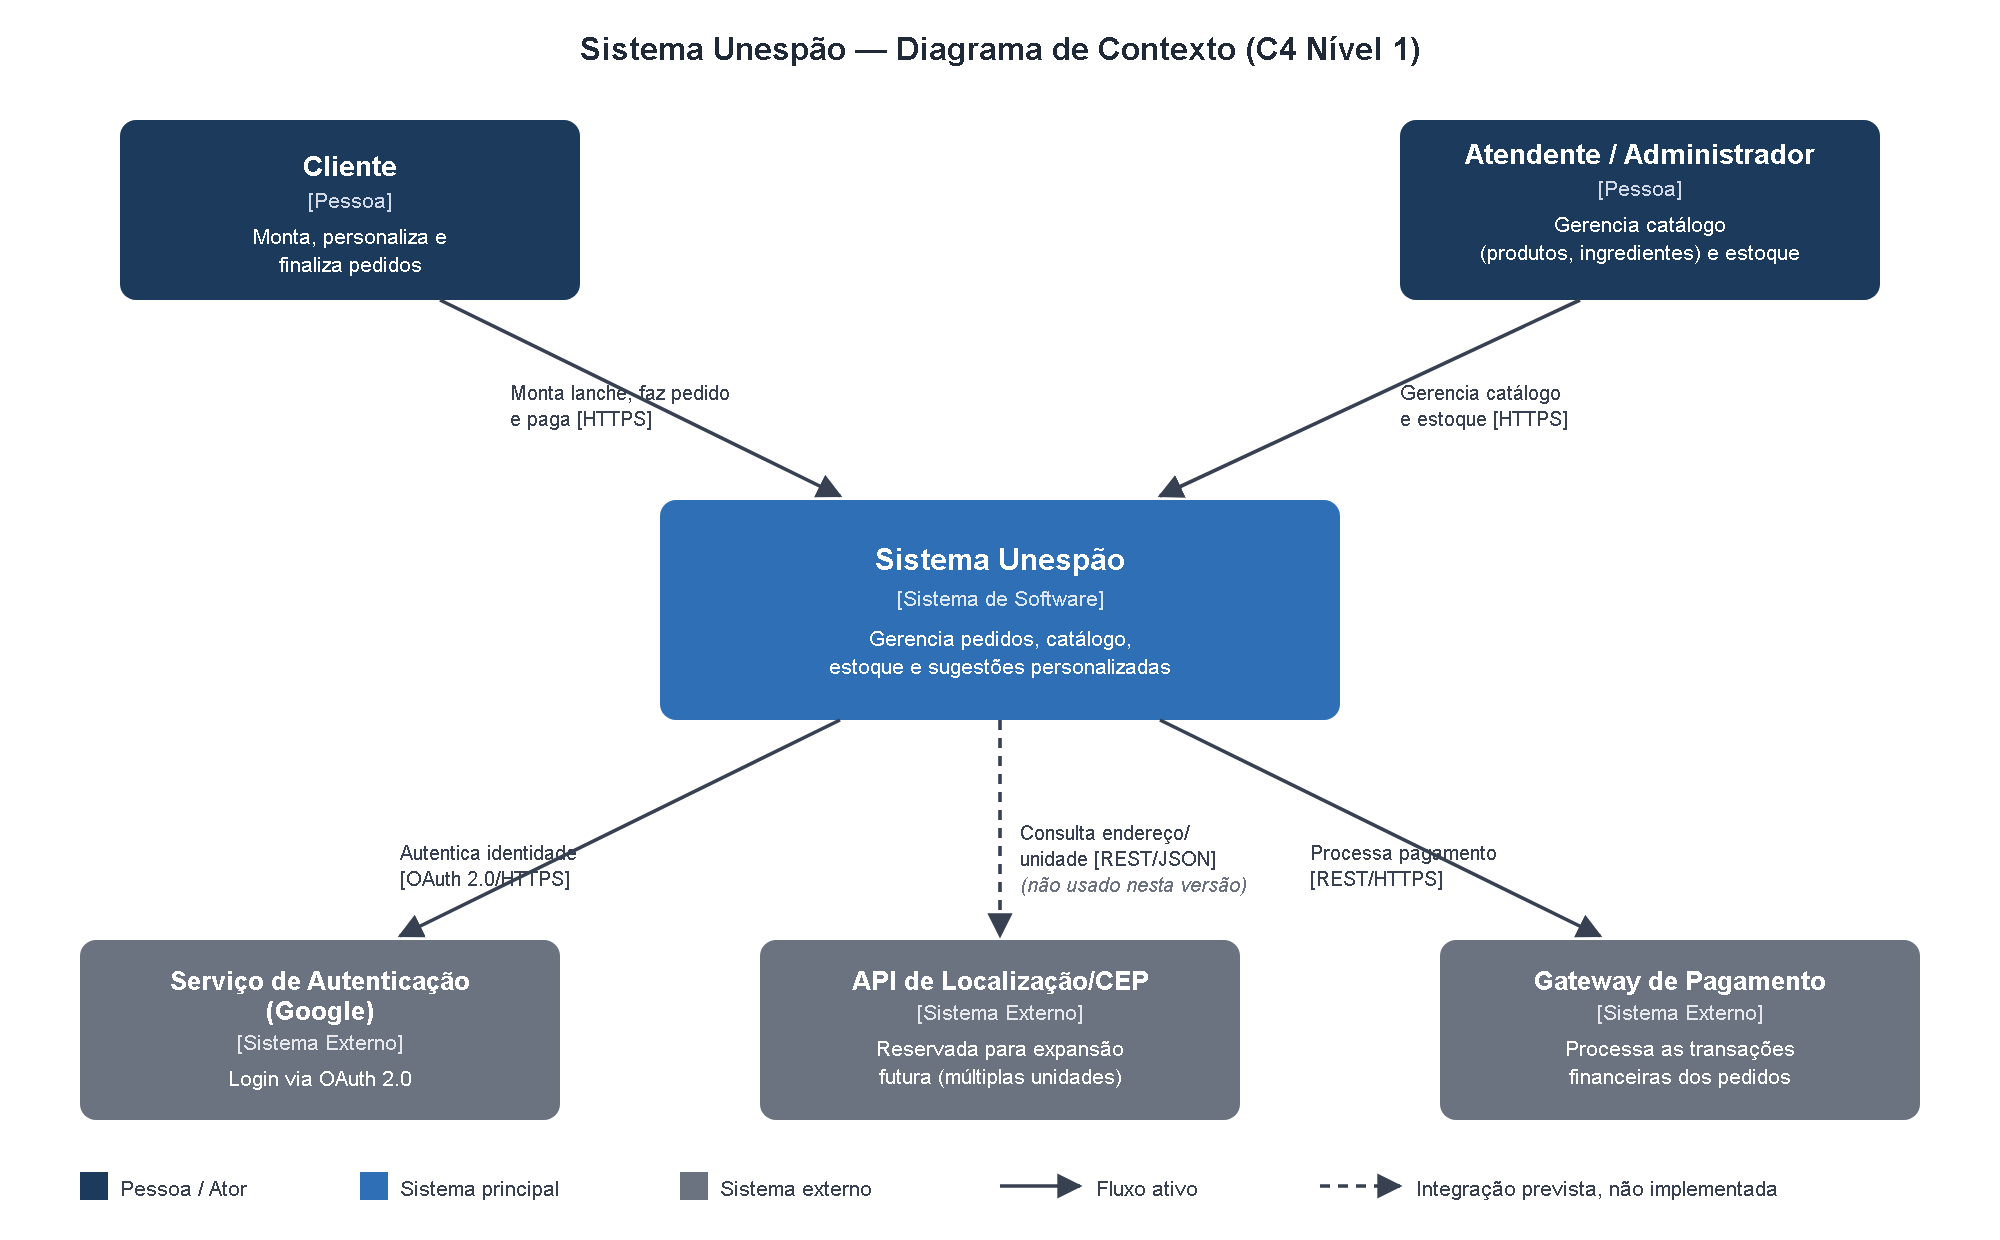
\includegraphics[width=0.95\textwidth]{c4-nivel1-contexto.png}
\caption{Diagrama de Contexto do Sistema Unespão (C4 Nível 1), já com os dois atores humanos do sistema.}
\label{fig:c4-contexto}
\end{figure}

A Figura~\ref{fig:c4-contexto} traz o diagrama de contexto (C4 Nível 1), que trata o sistema como uma caixa preta e mostra apenas quem interage com ele de fora. Nela aparecem dois atores humanos -- o Cliente, que monta, personaliza e finaliza pedidos, e o Atendente/Administrador da padaria, responsável pela gestão de catálogo (produtos base e ingredientes) e de estoque --, o próprio Sistema Unespão, e três sistemas externos com os quais ele troca informação: o Serviço de Autenticação do Google, a API de Localização/CEP e o Gateway de Pagamento. O diagrama também indica os protocolos de cada relação -- o cliente fala com o sistema via HTTPS, e o sistema, por sua vez, usa HTTPS/OAuth 2.0 para autenticar o cliente junto ao Google, REST/JSON para consultar a API de CEP e REST/HTTPS para acionar o gateway de pagamento. Em resumo, a lógica de negócio inteira mora dentro da caixa ``Sistema Unespão''; os três sistemas externos são fornecedores de capacidades específicas (identidade, endereço, dinheiro) que o Unespão consome, nunca o contrário.

O sistema modela uma única loja da padaria Unespão, não uma rede de unidades. A API de Localização/CEP aparece no diagrama pensando numa expansão futura do produto -- o dia em que a Unespão eventualmente abrir mais lojas e precisar direcionar o cliente para a unidade correta --, mas hoje ela permanece fora de uso efetivo; sua menção fica registrada no diagrama para essa eventualidade.

Ficam fora das fronteiras do sistema, por decisão de escopo do grupo: a logística de entrega (o modelo é de retirada na própria loja, via totem ou app, sem fluxo de delivery); a gestão financeira e contábil da padaria como negócio (o sistema processa o pagamento pontual de cada pedido através do gateway, mas não é um sistema de fluxo de caixa ou contabilidade); a gestão de funcionários e recursos humanos (folha de pagamento, escalas de trabalho); e o atendimento presencial que eventualmente aconteça em paralelo ao canal digital, por ser operação humana da padaria e não uma funcionalidade de software.

\section{Estilo ou padrão arquitetural}

Optamos por Clean Architecture, organizada como uma arquitetura em camadas com fluxo unidirecional de dependências. Na prática, o backend é dividido em camadas concêntricas -- Controllers, Services, Repositories/External Adapters e Domain Models -- e cada camada só pode depender da camada imediatamente abaixo dela, nunca o contrário. As entidades de domínio (Cliente, Pedido, Estoque, e assim por diante) não conhecem nenhuma camada superior; quem depende delas são os repositórios e os serviços, não o inverso.

A escolha está ligada aos objetivos de qualidade definidos no capítulo de Introdução. A confiabilidade da informação de estoque, por exemplo, exige que a lógica de baixa de insumos fique concentrada num único lugar e não espalhada por controllers ou por chamadas ad hoc ao banco -- é o que o Princípio da Responsabilidade Única (SRP) garante ao isolar essa lógica dentro de um \texttt{EstoqueService} dedicado, único ponto do sistema autorizado a decidir como o estoque é debitado após um pedido. Já o objetivo de segurança dos dados e das transações do cliente se apoia no Princípio da Inversão de Dependência (DIP): os serviços de negócio, como o \texttt{PedidoService}, dependem apenas de interfaces (\texttt{IGatewayPagamentoAdapter}, \texttt{IPedidoRepository}) e nunca de implementações concretas, o que mantém credenciais de integrações externas -- tokens do Google, chaves do gateway de pagamento -- isoladas dentro dos adapters, sem vazamento para as camadas de negócio.

O capítulo de Projeto de Componentes retoma cada princípio SOLID com mais profundidade, classe por classe; aqui a escolha aparece como decisão de alto nível porque orienta a arquitetura descrita nas seções seguintes.

\section{Contêineres e componentes}

\begin{figure}[H]
\centering
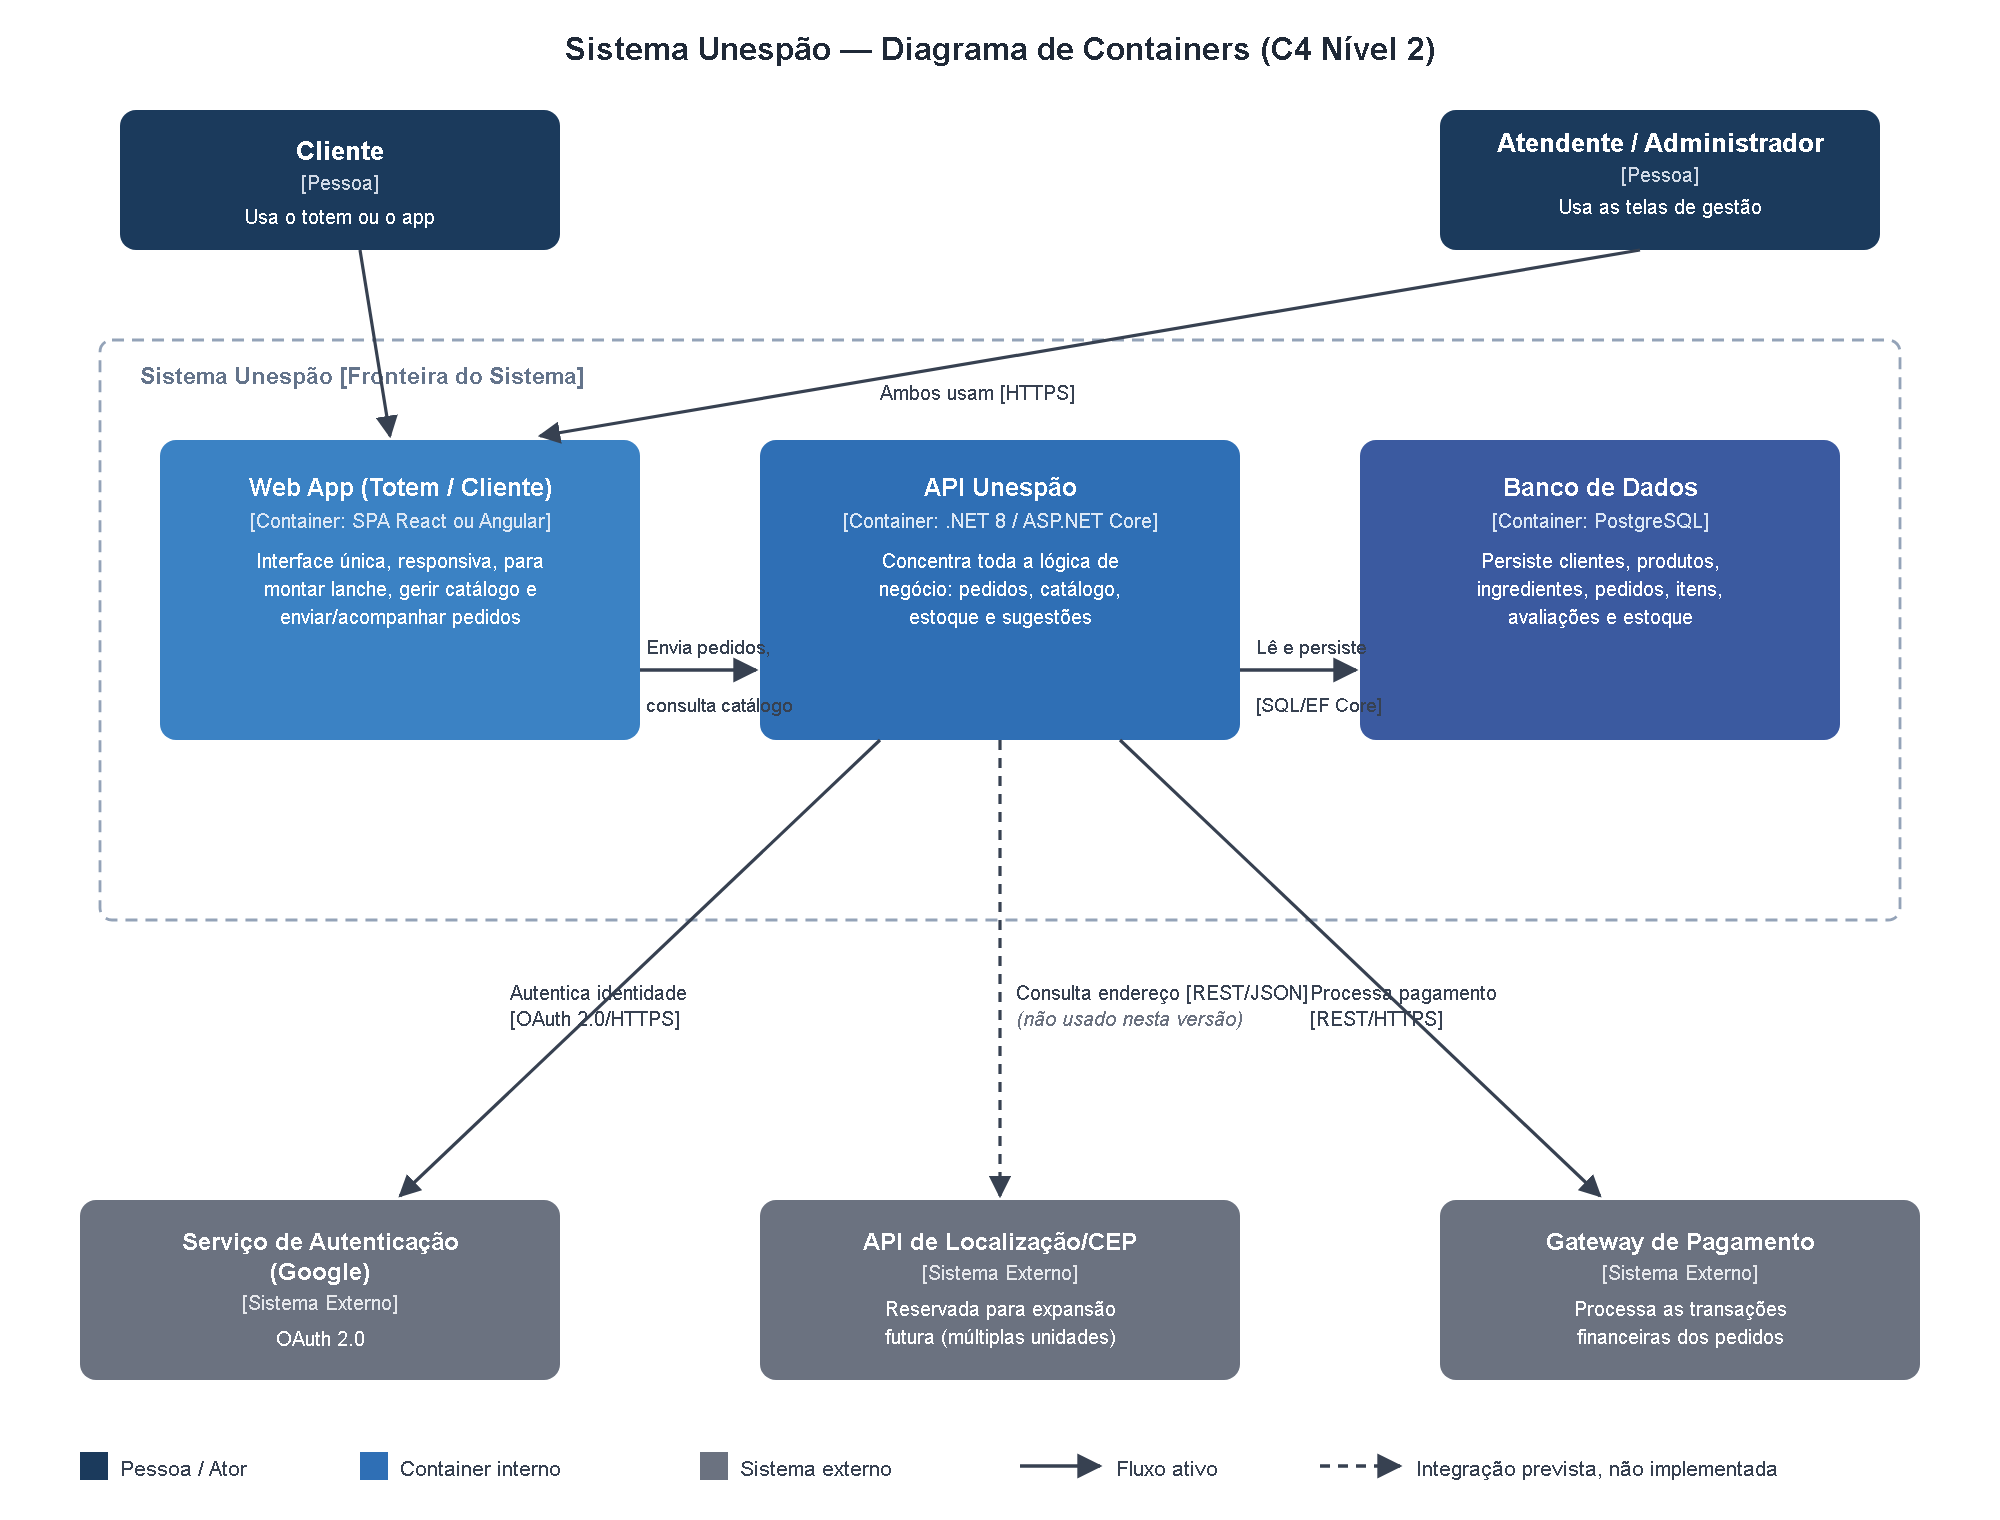
\includegraphics[width=0.95\textwidth]{c4-nivel2-containers.png}
\caption{Diagrama de Containers do Sistema Unespão (C4 Nível 2).}
\label{fig:c4-containers}
\end{figure}

A Figura~\ref{fig:c4-containers} mostra o diagrama de containers (C4 Nível 2), que abre a caixa preta do diagrama anterior e revela as três peças tecnológicas que formam o Sistema Unespão.

O primeiro container é o Web App (Totem e Cliente): um único SPA construído em React, rodando em modo responsivo tanto na tela do totem físico quanto no navegador do cliente, sem app móvel separado nem código duplicado entre os dois pontos de acesso. É essa mesma interface, adaptada ao tamanho de tela de cada dispositivo, que tanto o Cliente quanto o Atendente/Administrador usam, com permissões diferenciadas por perfil controladas pela API: o Cliente monta o lanche, consulta o cardápio disponível (já refletindo o estoque) e finaliza o pedido, enquanto o Atendente/Administrador acessa as telas de gestão de catálogo e de estoque. O segundo container é a API Unespão, escrita em .NET 8 com ASP.NET Core, que concentra toda a lógica de negócio do sistema -- cadastro de produtos e ingredientes, composição de itens personalizados, controle de estoque, cancelamento ou edição de item do pedido antes da confirmação do pagamento, histórico de pedidos e geração de sugestões personalizadas. O terceiro é o banco de dados PostgreSQL, responsável por persistir clientes, produtos base, ingredientes, pedidos, itens personalizados, avaliações e estoque.

A comunicação entre esses containers segue um padrão importante para a segurança do sistema: o Web App fala com a API Unespão via HTTPS/JSON, e é só a API que acessa o banco (via Entity Framework Core com o provider Npgsql) e que se comunica com os três sistemas externos do diagrama de contexto. Nem o Google Auth, nem a API de CEP, nem o gateway de pagamento são acessados diretamente pelo frontend -- toda integração externa passa pela API, que guarda tokens e credenciais fora do alcance do navegador do cliente, viabilizando o objetivo de segurança mencionado na seção anterior.

Do ponto de vista de componentes internos da API (C4 Nível 3, detalhado no capítulo de Projeto de Componentes), a organização segue seis grupos alinhados ao estilo em camadas: Controllers na porta de entrada HTTP, Services concentrando as regras de negócio, Repositories abstraindo a persistência, External Adapters isolando a comunicação com sistemas de terceiros, Domain Models representando as entidades ricas do domínio, e a camada de Infrastructure (o \texttt{UnespaoDbContext}) mapeando esses modelos para o esquema relacional do PostgreSQL.

\section{Decisões arquiteturais relevantes}

\begin{table}[H]
\centering
\caption{Decisões arquiteturais relevantes do Sistema Unespão.}
\begin{tabularx}{0.95\textwidth}{p{0.24\textwidth} X X}
\toprule
\textbf{Decisão} & \textbf{Motivação} & \textbf{Consequências} \\
\midrule
Adotar Clean Architecture / arquitetura em camadas com fluxo unidirecional de dependências & Isolar a lógica de negócio de detalhes de infraestrutura, facilitando testes e reduzindo o custo de trocar uma peça tecnológica sem afetar as demais. & Mais interfaces e classes de mapeamento entre camadas; em compensação, cada camada é testável isoladamente e trocar banco ou gateway fica restrito a Repositories e External Adapters. \\
Centralizar toda comunicação com sistemas externos na API Unespão, nunca no frontend & Evitar que tokens de autenticação e credenciais de pagamento fiquem expostos no navegador/totem do cliente. & Todo fluxo de autenticação e pagamento passa por uma chamada adicional ao backend, o que acrescenta uma etapa de rede mas concentra a superfície de segurança em um único ponto auditável. \\
Usar um único SPA responsivo em React em vez de app móvel nativo separado (ver seção de Contêineres) & Atender totem e navegador do cliente com o mesmo frontend e backend, sem duplicar código nem manter duas bases de código para as mesmas telas. & Toda regra de negócio fica no backend, evitando inconsistência entre o que aparece no totem e no navegador. \\
Modelar uma loja única, mantendo a API de CEP mapeada na arquitetura como capacidade de expansão (ver seção de Contexto) & O escopo do produto é uma padaria de unidade única; o roteamento entre lojas não é um problema deste sistema. & A arquitetura já reserva o ponto de integração para quando a rede de lojas crescer, sem exigir redesenho do contexto nessa expansão futura. \\
Isolar a lógica de estoque em um EstoqueService dedicado (SRP) & Garantir a confiabilidade da informação de estoque, objetivo de qualidade de prioridade alta definido na Introdução. & Único ponto de responsabilidade para a baixa de insumos, reduzindo o risco de inconsistência entre o cardápio exibido e o estoque físico. \\
Depender de abstrações nos serviços de negócio, isolando credenciais nos External Adapters (DIP) & Suportar a segurança dos dados e transações do cliente sem acoplar a lógica de pedido a uma implementação específica de gateway ou autenticação. & Facilita testes com dependências fake e permite trocar/adicionar um gateway de pagamento criando um novo adapter, sem alterar o PedidoService. \\
\bottomrule
\end{tabularx}
\end{table}

\section{Restrições de arquitetura}

A stack tecnológica já está definida e não é objeto de discussão neste projeto: backend em .NET 8 com ASP.NET Core, persistência em PostgreSQL e o frontend SPA descrito na seção de Contêineres. Trata-se de uma restrição herdada da documentação arquitetural produzida anteriormente pelo próprio grupo e mantida como decisão de projeto consolidada.

O sistema é desenvolvido no contexto da disciplina de Engenharia de Software II, na UNESP, o que traz restrições próprias de um trabalho acadêmico: prazo de entrega fixo dentro do semestre letivo, equipe pequena e sem dedicação exclusiva ao projeto, e a exigência de que a documentação evidencie explicitamente os conceitos vistos em aula (Modelo C4, princípios SOLID, entre outros), não apenas o funcionamento do software em si.

Há também três restrições de integração obrigatórias, não triviais de contornar sem redesenhar a arquitetura: autenticação via Google OAuth 2.0, processamento financeiro via gateway de pagamento externo, e a API de CEP reservada para a expansão a múltiplas lojas já discutida nas seções anteriores. As três partem exclusivamente da API Unespão, nunca do frontend, pela mesma decisão de segurança da tabela acima.

% ============================================================================
\chapter{Projeto de Componentes}
% ============================================================================

\section{Visão geral dos componentes}

A API Unespão (.NET 8 / ASP.NET Core) é o único container que concentra lógica de negócio no sistema: o Web App/Totem funciona apenas como camada de apresentação, e o banco PostgreSQL só é acessado através dela. Internamente essa API está organizada em seis grupos de componentes, com fluxo de dependência unidirecional -- Controllers chamam Services, que por sua vez dependem de Repositories e de External Adapters; ambos operam sobre os Domain Models, e a persistência efetiva passa pela camada de Infrastructure (DbContext). Essa organização segue os princípios de Clean Architecture: cada camada conhece apenas a camada imediatamente abaixo dela, e os Domain Models não dependem de nenhuma outra camada.

A tabela a seguir resume os componentes e suas responsabilidades.

\begin{table}[H]
\centering
\caption{Principais componentes da API Unespão.}
\begin{tabularx}{0.95\textwidth}{p{0.30\textwidth} X}
\toprule
\textbf{Componente} & \textbf{Responsabilidade principal} \\
\midrule
Controllers (\texttt{ClientesController}, \texttt{PedidosController}, \texttt{ProdutosController}, \texttt{AvaliacoesController}, \texttt{EstoqueController}) & Receber requisições HTTP do frontend, validar dados de entrada, delegar a execução aos serviços apropriados e devolver respostas em JSON. Não contêm regra de negócio. \\
Services (\texttt{ClienteService}, \texttt{ProdutoService}, \texttt{PedidoService}, \texttt{AvaliacaoService}, \texttt{EstoqueService}, \texttt{SugestaoPersonalizadaService}) & Concentrar a lógica de domínio, coordenar chamadas a repositórios e adapters externos e garantir a consistência de operações que envolvem mais de uma entidade (por exemplo, criar um pedido e dar baixa no estoque). \\
Repositories (\texttt{IRepository<T>} e as interfaces específicas \texttt{IClienteRepository}, \texttt{IPedidoRepository}, \texttt{IProdutoRepository}, \texttt{IAvaliacaoRepository}, \texttt{IEstoqueRepository}, com suas implementações concretas) & Abstrair o acesso a dados, expondo uma interface padronizada de operações CRUD sobre as entidades de domínio, usando Entity Framework Core e o provider Npgsql. \\
External Adapters (\texttt{GoogleAuthAdapter}, \texttt{LocalizacaoAdapter}, \texttt{GatewayPagamentoAdapter}) & Isolar a comunicação com sistemas externos (autenticação Google, consulta de CEP e gateway de pagamento), traduzindo o formato exigido por cada API externa para o modelo interno da aplicação. \\
Domain Models (\texttt{Cliente}, \texttt{ProdutoBase}, \texttt{Ingrediente}, \texttt{ItemPersonalizado}, \texttt{Pedido}, \texttt{AvaliacaoPrato}, \texttt{Estoque}) & Representar as entidades de negócio e suas regras, sem depender de nenhuma outra camada da aplicação. \\
Infrastructure (\texttt{UnespaoDbContext}) & Mapear os Domain Models para o esquema relacional do PostgreSQL e gerenciar a conexão com o banco via Entity Framework Core. \\
\bottomrule
\end{tabularx}
\end{table}

Do ponto de vista de quem usa o sistema, os dois atores do minimundo acionam grupos distintos de Controllers: o Cliente interage com \texttt{ClientesController}, \texttt{PedidosController} e \texttt{AvaliacoesController} (cadastro, autenticação, montagem/edição de pedido personalizado, pagamento e avaliação de pratos); já o Atendente/Administrador da padaria -- ator de perfil mais simples, responsável pelo CRUD de catálogo e estoque -- opera por meio de \texttt{ProdutosController} e \texttt{EstoqueController}. Essa separação de Controllers por ator já reflete, na camada de apresentação da API, a distinção de perfis que motiva a existência do \texttt{EstoqueService} como ponto único de manipulação de estoque, detalhado na seção seguinte.

Optamos por manter essa granularidade, com camadas bem definidas em vez de uma organização mais ``achatada'', porque ela conversa diretamente com dois dos objetivos de qualidade definidos no capítulo de Introdução. Um é a confiabilidade da informação de estoque, que depende de a lógica de baixa de insumos estar concentrada e isolada em um único componente (\texttt{EstoqueService}). O outro é a segurança dos dados e transações do cliente, que exige que credenciais de terceiros (Google, gateway de pagamento) fiquem restritas aos Adapters e nunca cheguem ao frontend.

\section{Detalhamento dos componentes principais}

Dos seis grupos, três concentram a maior parte da complexidade e do risco de mudança do sistema: os Services, os Repositories e os External Adapters. É neles que detalhamos a seguir responsabilidades, interfaces e dependências. Como o Sistema Unespão é um projeto orientado a objetos, o diagrama de classes UML simplificado abaixo resume os grupos de componentes e as principais interfaces e dependências entre eles; o texto que segue detalha cada um.

\begin{figure}[H]
\centering
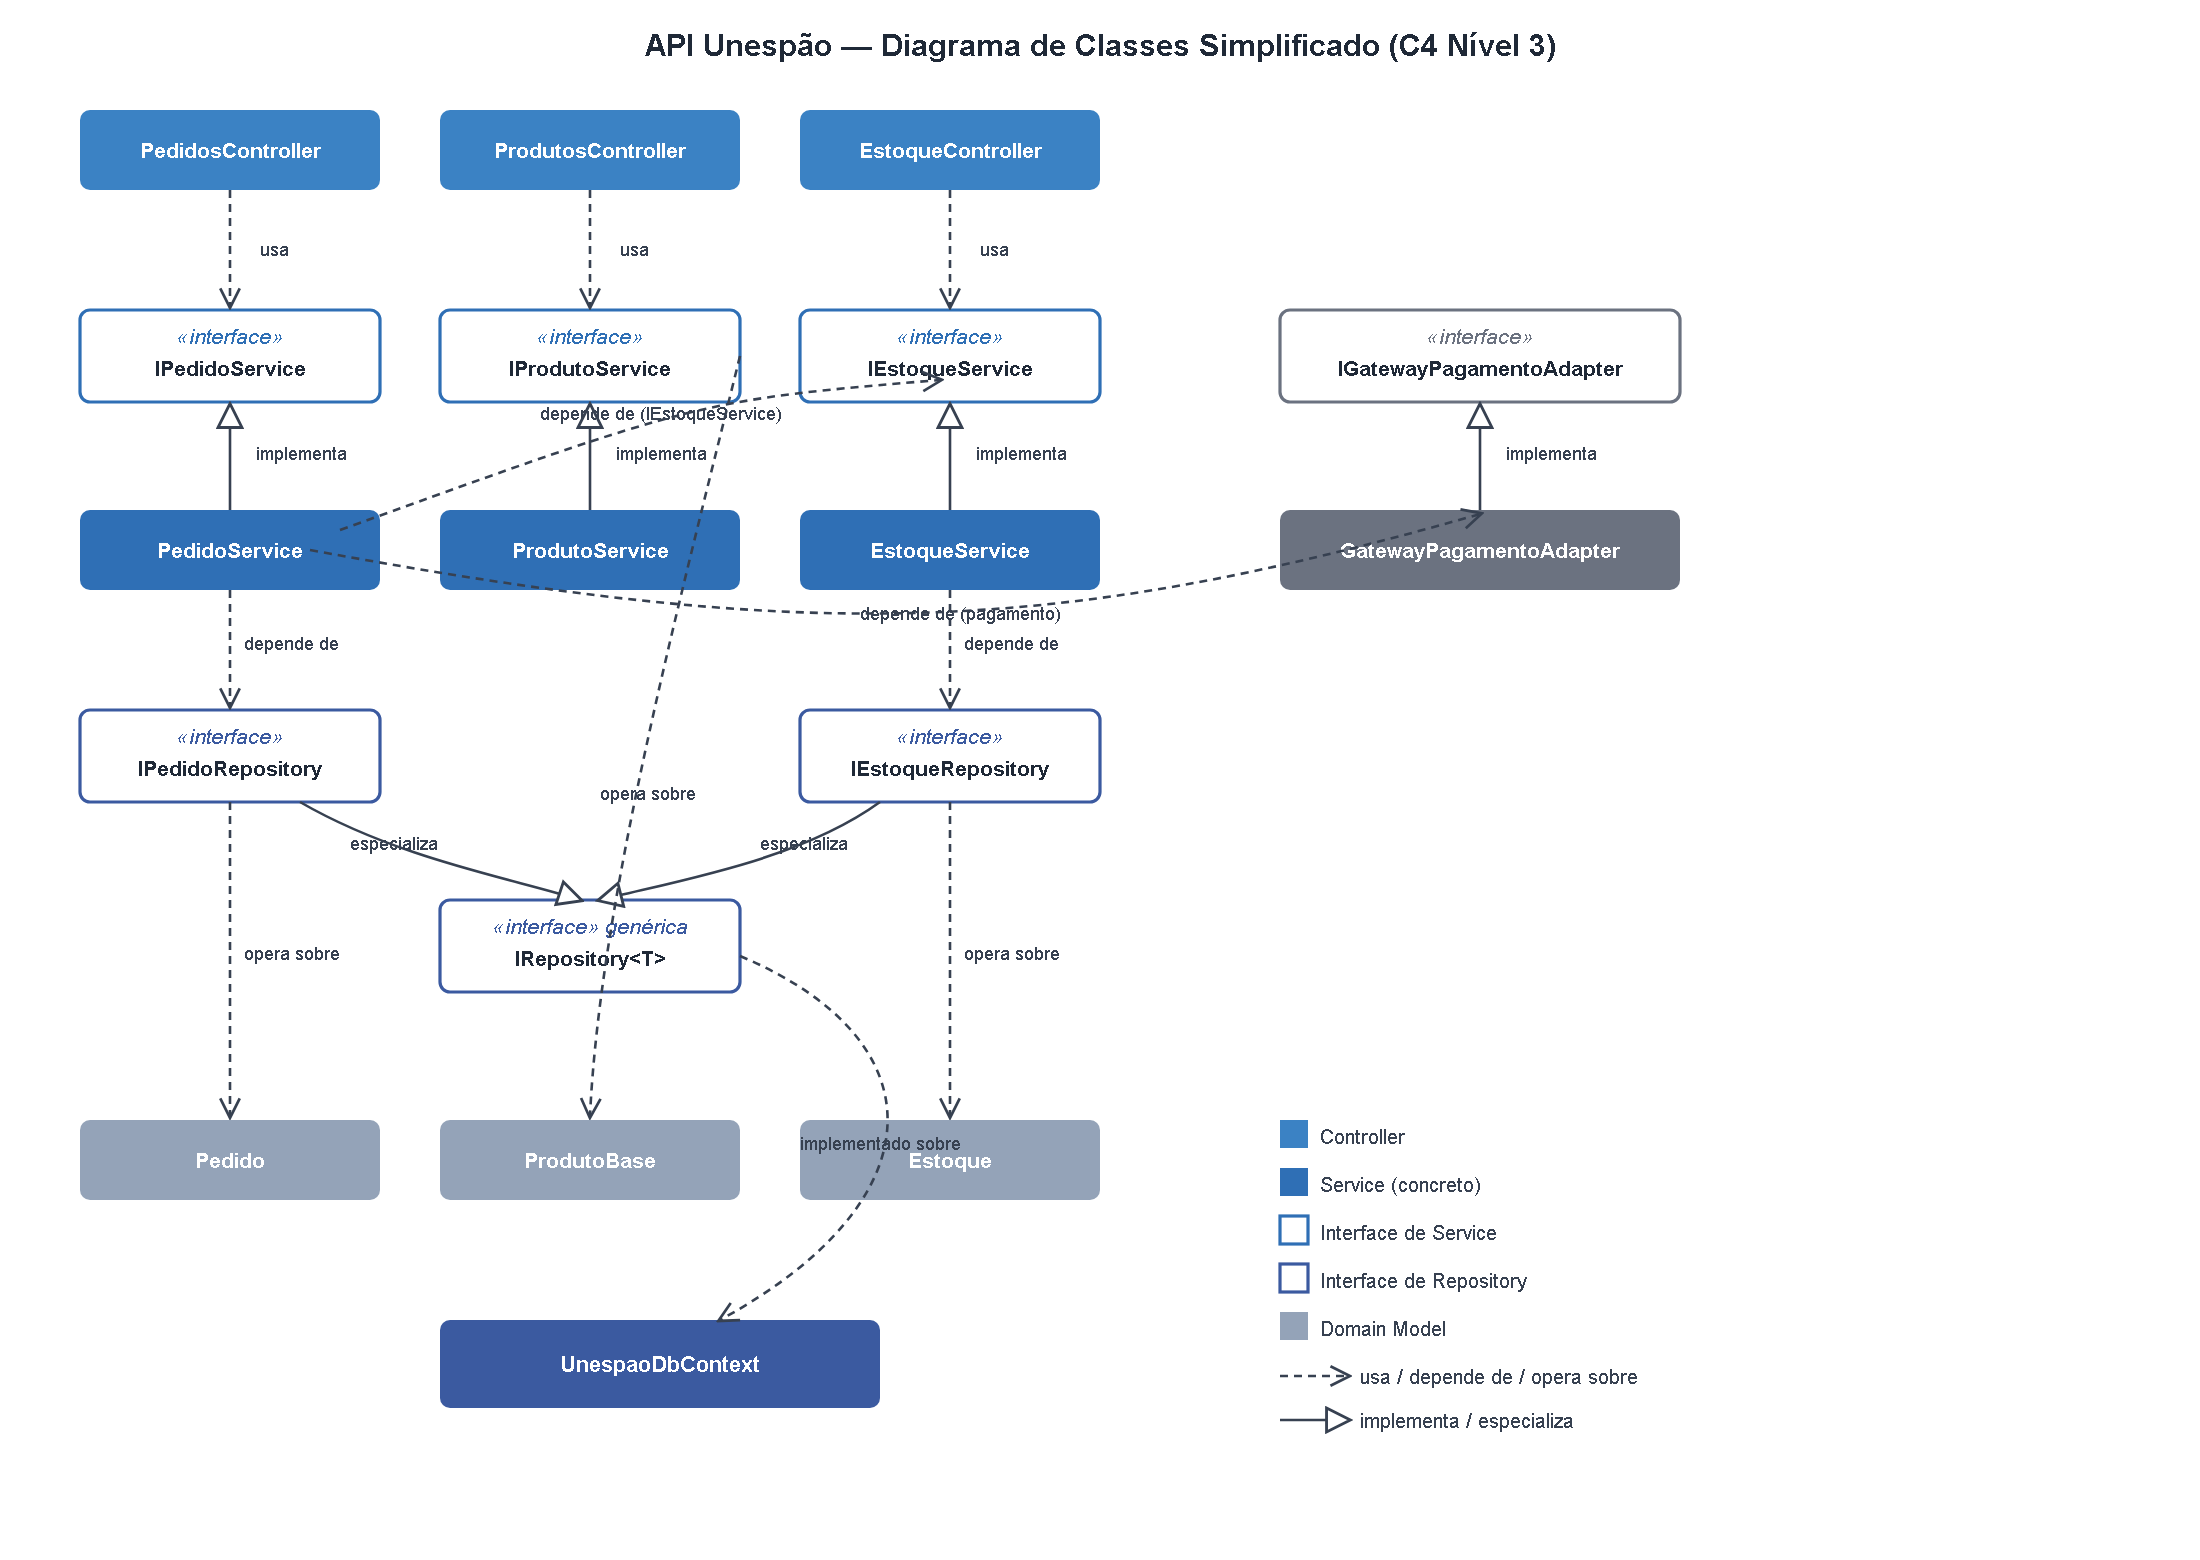
\includegraphics[width=0.95\textwidth]{c4-nivel3-diagrama-classes.png}
\caption{Diagrama de classes simplificado da API Unespão (C4 Nível 3), com os grupos de componentes mais relevantes e suas dependências.}
\label{fig:diagrama-classes}
\end{figure}

Na leitura do diagrama, as setas tracejadas com ponta aberta (``usa''/``depende de'') indicam dependência em tempo de execução via injeção de construtor, enquanto as setas de implementação de interface ligam cada Service à sua abstração correspondente -- é essa cadeia (Controller $\rightarrow$ interface de Service $\rightarrow$ Service concreto $\rightarrow$ interface de Repository/Adapter) que materializa a Clean Architecture descrita na seção anterior: nenhuma seta cruza diretamente para uma classe concreta de outra camada.

\textbf{PedidoService.} É o componente mais crítico do sistema, pois orquestra o ciclo de vida completo de um pedido: criação, edição ou cancelamento de itens antes da confirmação de pagamento (requisito adotado pelo grupo), personalização dos itens e processamento do pagamento. Suas dependências são todas abstrações -- \texttt{IPedidoRepository}, \texttt{IEstoqueService} e \texttt{IGatewayPagamentoAdapter} -- nunca as classes concretas correspondentes. Essa decisão não é incidental: é o que permite trocar o gateway de pagamento ou substituir o repositório por uma versão em memória nos testes sem tocar em uma linha do serviço.

Para tornar concreto esse fluxo de criação/confirmação de pedido -- o mais crítico do sistema --, o diagrama de sequência a seguir mostra a interação entre \texttt{PedidosController}, \texttt{PedidoService} e as abstrações que ele consome, sem detalhar o Domain Model interno:

\begin{figure}[H]
\centering
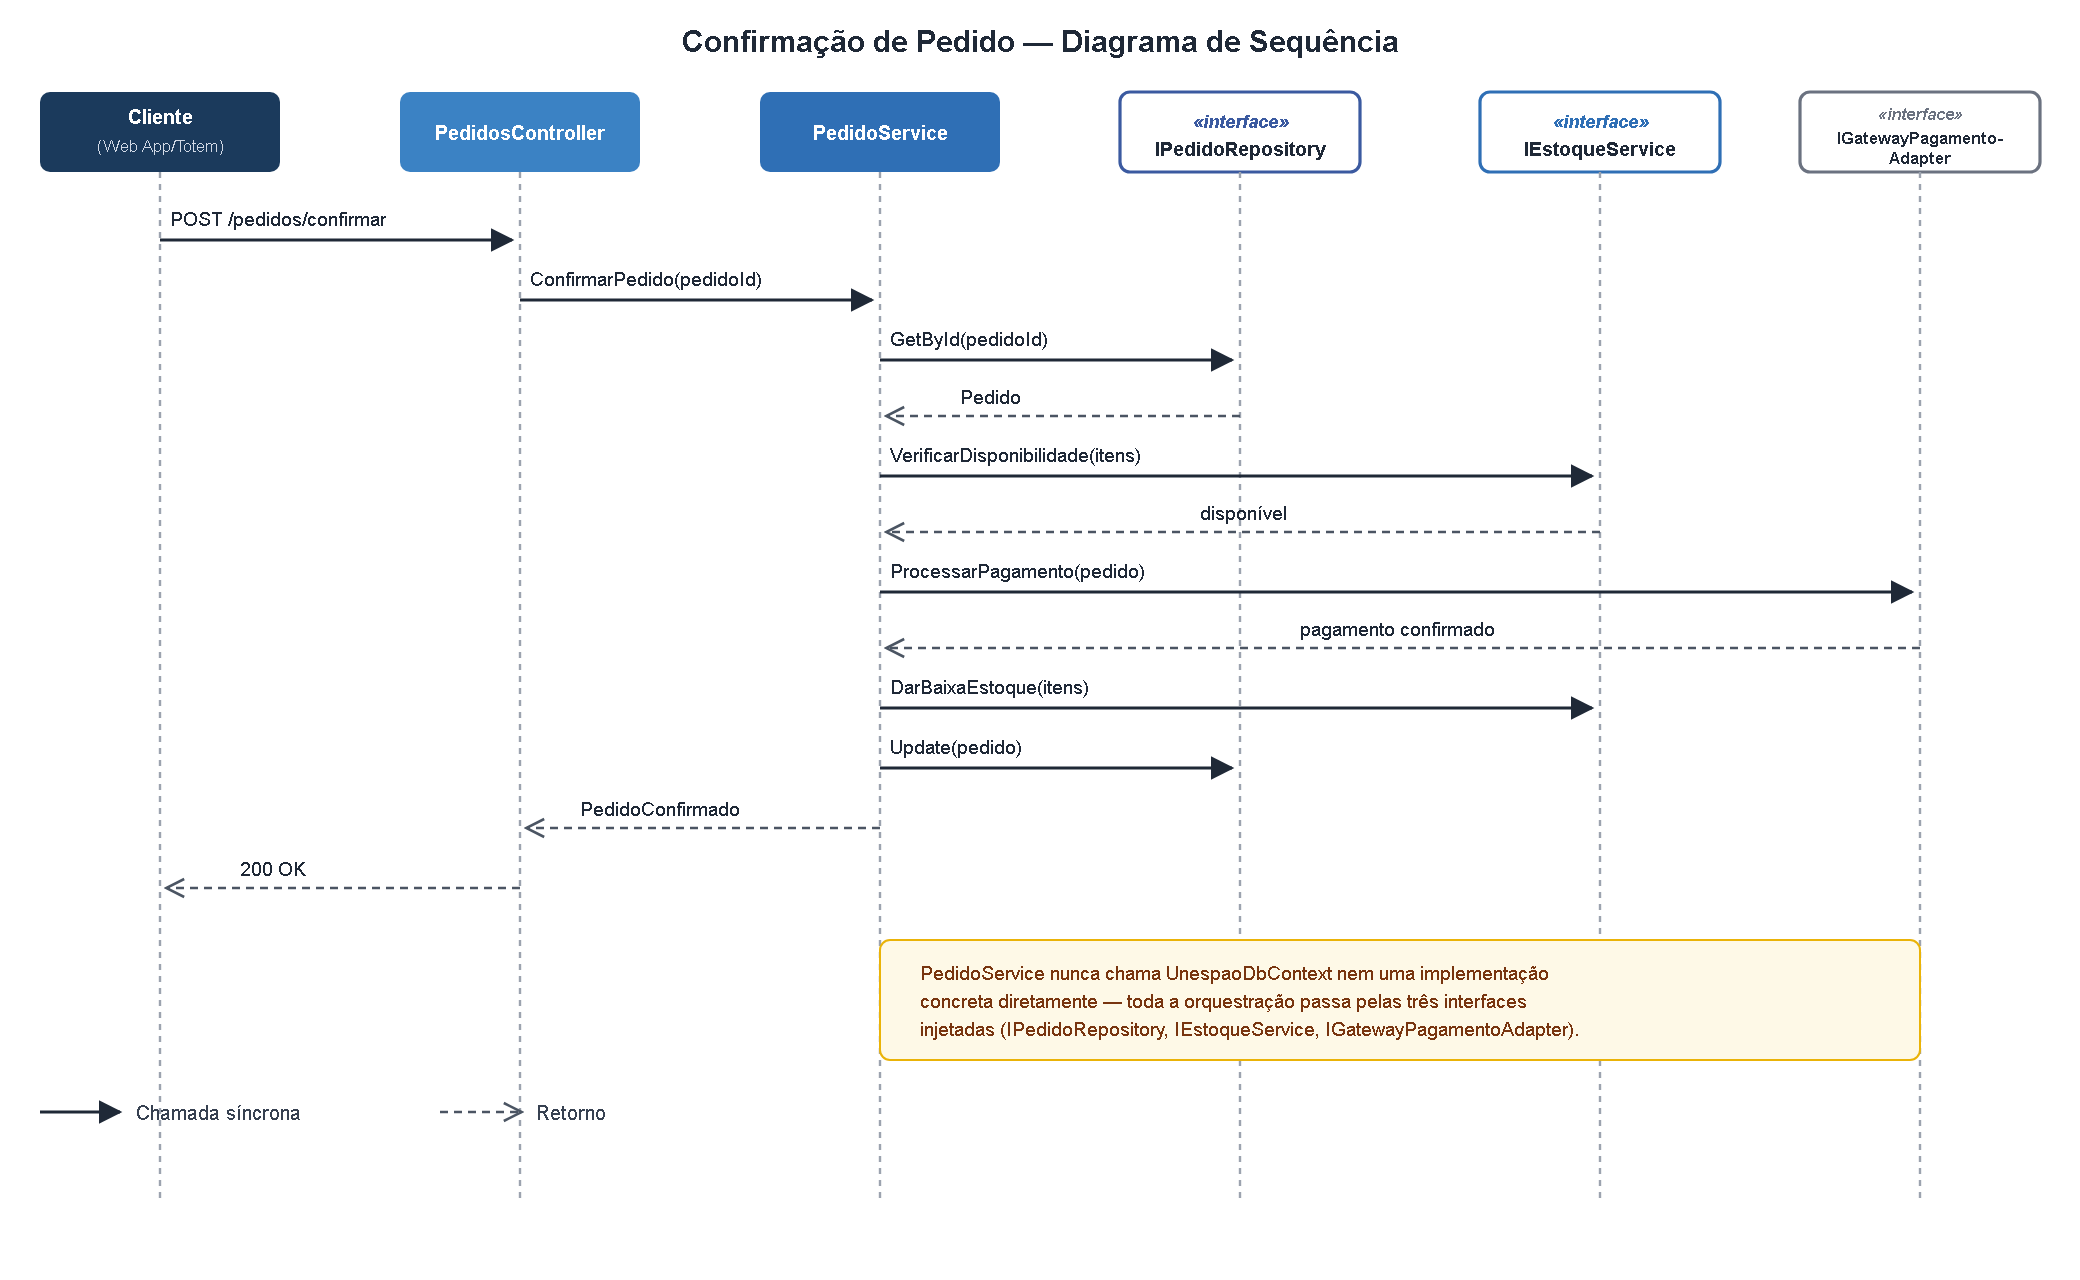
\includegraphics[width=0.95\textwidth]{diagrama-sequencia-confirmar-pedido.png}
\caption{Diagrama de sequência da confirmação de pedido, do \texttt{PedidosController} até as três interfaces que o \texttt{PedidoService} orquestra.}
\label{fig:diagrama-sequencia}
\end{figure}

O diagrama evidencia que \texttt{PedidoService} nunca chama diretamente o \texttt{UnespaoDbContext} nem uma implementação concreta de gateway: toda a orquestração passa pelas três interfaces injetadas, o que é o que possibilita, por exemplo, substituir \texttt{GatewayPagamentoAdapter} por um dublê de teste sem alterar essa sequência de chamadas.

\textbf{EstoqueService.} Cuida exclusivamente da disponibilidade de produtos base e ingredientes, incluindo a baixa de insumos quando um pedido é confirmado. A separação desse componente do \texttt{PedidoService} é uma decisão deliberada de projeto: como o objetivo de qualidade ``confiabilidade da informação de estoque'' tem prioridade alta, isolar essa lógica em uma única classe reduz a chance de uma alteração na regra de pedidos afetar, por efeito colateral, o controle de estoque, e vice-versa. Na leitura do grupo, esse componente também é o ponto natural de extensão para os requisitos de CRUD de catálogo e estoque operados pelo Atendente/Administrador: as operações de cadastro e ajuste de estoque desse ator, expostas via \texttt{ProdutosController} e \texttt{EstoqueController}, passam pelo mesmo \texttt{EstoqueService}, e não por um caminho paralelo.

\textbf{IRepository<T> e as implementações concretas.} A camada de Repositories é construída sobre uma interface genérica, \texttt{IRepository<T>}, que define as operações CRUD comuns a todas as entidades, complementada por interfaces específicas (\texttt{IClienteRepository}, \texttt{IPedidoRepository} etc.) que acrescentam métodos próprios do domínio, como \texttt{GetClienteWithHistorico}. Cada Service depende apenas da interface, nunca da implementação concreta que fala com o PostgreSQL, o que possibilita a existência de implementações alternativas para teste, como \texttt{MockPedidoRepository}, discutida na seção seguinte. Essa relação de especialização (\texttt{IPedidoRepository} e \texttt{IEstoqueRepository} estendendo \texttt{IRepository<T>}) é exatamente o que o diagrama de classes acima representa pelas setas de generalização entre essas interfaces.

\textbf{External Adapters.} \texttt{GoogleAuthAdapter}, \texttt{LocalizacaoAdapter} e \texttt{GatewayPagamentoAdapter} encapsulam, cada um, a comunicação com um sistema externo específico do C4 Nível 1 (Serviço de Autenticação Google, API de Localização/CEP e Gateway de Pagamento, respectivamente). Como já vale para os Repositories, cada adapter é acessado pelos Services por meio de uma interface própria (\texttt{IGoogleAuthAdapter}, \texttt{ILocalizacaoAdapter}, \texttt{IGatewayPagamentoAdapter}), nunca pela classe concreta -- é essa abstração que o \texttt{ClienteService} consome ao delegar a validação do token do Google ao \texttt{GoogleAuthAdapter} por trás de \texttt{IGoogleAuthAdapter}, no mesmo espírito do DIP já discutido para \texttt{IGatewayPagamentoAdapter} na seção de Princípios de projeto. Nenhum deles é chamado diretamente pelo frontend: a API Unespão sempre medeia essas integrações, o que mantém tokens e credenciais fora do navegador do cliente. Vale registrar que, como decidido no escopo do produto, a API de Localização/CEP é um recurso pensado para uma futura expansão a múltiplas unidades; no escopo atual, de loja única, o \texttt{LocalizacaoAdapter} existe na arquitetura mas não tem uso funcional imediato.

\textbf{UnespaoDbContext.} Fecha o fluxo de dependências mapeando os Domain Models para o esquema relacional via Entity Framework Core, expondo um \texttt{DbSet<>} para cada entidade persistente (Clientes, ProdutosBase, Ingredientes, Pedidos, ItensPersonalizados, AvaliacoesPrato e Estoque). É o único ponto do sistema que conhece o dialeto do PostgreSQL; substituir o banco de dados por outro SGBD afetaria, em tese, apenas essa classe e as implementações concretas dos Repositories.

\section{Princípios de projeto}

Os cinco princípios SOLID orientaram as decisões de projeto da API Unespão. Em vez de tratá-los como uma lista teórica, procuramos, para cada um, indicar o problema concreto de projeto que ele resolveu no sistema, complementando a análise com o trecho de código do construtor de \texttt{PedidoService} a seguir, que evidencia de forma direta a aplicação de DIP e ISP:

\begin{lstlisting}[language=csharp, caption={Construtor de \texttt{PedidoService}, com suas três dependências expressas como interfaces.}]
public class PedidoService : IPedidoService
{
    private readonly IPedidoRepository _pedidoRepository;
    private readonly IEstoqueService _estoqueService;
    private readonly IGatewayPagamentoAdapter _gatewayPagamento;

    public PedidoService(
        IPedidoRepository pedidoRepository,
        IEstoqueService estoqueService,
        IGatewayPagamentoAdapter gatewayPagamento)
    {
        _pedidoRepository = pedidoRepository;
        _estoqueService = estoqueService;
        _gatewayPagamento = gatewayPagamento;
    }

    // ConfirmarPedido, AdicionarItem, RemoverItem, etc.
}
\end{lstlisting}

Nenhum dos três parâmetros do construtor é uma classe concreta (\texttt{PedidoRepository}, \texttt{EstoqueService} ou \texttt{GatewayPagamentoAdapter}): todos são interfaces, resolvidas em tempo de execução pelo container de injeção de dependência do ASP.NET Core. É esse trecho -- junto do diagrama de classes da seção anterior -- que sustenta concretamente as discussões de DIP e ISP abaixo.

\textbf{Responsabilidade única (SRP).} Cada Service tem um único motivo para mudar. \texttt{PedidoService} cuida só do ciclo de vida do pedido; \texttt{EstoqueService}, só de estoque e baixa de insumos; \texttt{AvaliacaoService}, só de feedback de pratos; \texttt{SugestaoPersonalizadaService}, só de recomendações. O ganho prático é direto: se a regra de pontuação de uma avaliação mudar, apenas \texttt{AvaliacaoService} é tocado, sem risco de regressão em pedidos ou estoque. Os Controllers seguem a mesma lógica, cada um respondendo a um conjunto coeso de endpoints.

\textbf{Aberto/fechado (OCP).} A interface genérica \texttt{IRepository<T>} permite acomodar novas entidades sem alterar código já existente, bastando criar uma nova implementação. O caso mais ilustrativo, porém, é o dos adapters de pagamento: trocar o gateway de Stripe por PagSeguro, ou adicionar suporte a Pix, significa criar uma nova classe que implementa \texttt{IGatewayPagamentoAdapter} -- o mesmo parâmetro \texttt{gatewayPagamento} do construtor acima passaria a receber outra implementação --, sem que \texttt{PedidoService} precise mudar uma única linha. Essa substituibilidade de gateways é a aplicação mais concreta de OCP no sistema, e é justamente o padrão Strategy que a sustenta -- retomamos esse ponto na seção de padrões de projeto.

\textbf{Substituição de Liskov (LSP).} Qualquer implementação de \texttt{IPedidoRepository} precisa poder substituir outra sem que \texttt{PedidoService} perceba diferença de comportamento. É o que garante, por exemplo, que \texttt{PedidoRepository} (a implementação real sobre PostgreSQL) e \texttt{MockPedidoRepository} (uma implementação em memória usada em teste) sejam intercambiáveis do ponto de vista do serviço que os consome -- ambas encaixam no mesmo parâmetro \texttt{pedidoRepository} do construtor. O cuidado aqui é que as implementações não podem quebrar as garantias do contrato: se \texttt{IPedidoRepository.GetById} promete devolver um \texttt{Pedido} válido, toda implementação precisa honrar isso, sob risco de falhas silenciosas em produção que só apareceriam ao trocar a implementação usada.

\textbf{Segregação de interfaces (ISP).} Em vez de uma interface única e genérica concentrando toda a lógica de serviço, o sistema define interfaces dedicadas -- \texttt{IClienteService}, \texttt{IPedidoService}, \texttt{IAvaliacaoService}, \texttt{IEstoqueService}, \texttt{ISugestaoPersonalizadaService} -- cada uma expondo apenas os métodos relevantes ao seu domínio. O mesmo raciocínio se aplica aos repositórios: \texttt{IRepository<T>} cobre o CRUD genérico, e interfaces como \texttt{IClienteRepository} acrescentam apenas os métodos específicos daquela entidade. O efeito é que cada Controller depende só do que usa (\texttt{ClientesController} não é forçado a conhecer métodos de estoque ou de pagamento), o que mantém o acoplamento baixo e permite que cada interface evolua de forma independente. No construtor de \texttt{PedidoService} isso aparece como três parâmetros estreitos e específicos (\texttt{IPedidoRepository}, \texttt{IEstoqueService}, \texttt{IGatewayPagamentoAdapter}), em vez de uma única interface genérica de ``serviços'' que agregasse métodos não usados por esse Service.

\textbf{Inversão de dependência (DIP).} \texttt{PedidoService} não conhece nenhuma classe concreta: suas dependências são sempre interfaces -- \texttt{IPedidoRepository}, \texttt{IEstoqueService}, \texttt{IGatewayPagamentoAdapter} --, exatamente como declarado no construtor acima, nunca \texttt{PedidoRepository}, \texttt{EstoqueService} ou \texttt{GatewayPagamentoAdapter} diretamente. Quem resolve essas dependências em tempo de execução é o container de injeção de dependência do ASP.NET Core, que registra as implementações concretas como provedoras de cada interface e as injeta no construtor de cada Service. Esse é, possivelmente, o princípio com maior impacto estrutural no projeto: é ele que sustenta a testabilidade (basta injetar uma implementação fake), a possibilidade de trocar o banco de dados afetando só a camada de Repositories, e o baixo acoplamento entre todas as camadas descritas na seção anterior.

\section{Padrões de projeto}

Documentamos aqui apenas os padrões cuja aplicação está de fato evidenciada na arquitetura do sistema.

\textbf{Repository.} Problema: a lógica de negócio dos Services não deveria depender diretamente de detalhes de acesso a dados (Entity Framework Core, SQL, provider Npgsql). Solução adotada: uma interface genérica \texttt{IRepository<T>} com as operações CRUD comuns, especializada por interfaces como \texttt{IPedidoRepository} e \texttt{IClienteRepository} para métodos próprios de cada entidade, cada uma com sua implementação concreta sobre PostgreSQL. Participantes: os Services (clientes do padrão), as interfaces de repositório e suas implementações concretas, e o \texttt{UnespaoDbContext} por trás delas. Benefício obtido: a lógica de negócio permanece isolada da tecnologia de persistência, e a substituição de uma implementação real por uma implementação de teste em memória (\texttt{MockPedidoRepository}) se torna possível sem alterar o código que a consome, o que viabiliza a estratégia de testes de unidade descrita no capítulo correspondente.

\textbf{Adapter.} Problema: o sistema precisa se comunicar com três serviços externos heterogêneos (autenticação Google via OAuth 2.0, API de Localização/CEP via REST/JSON, Gateway de Pagamento via REST/HTTPS), cada um com seu próprio protocolo e formato de dados, sem que essa heterogeneidade vaze para a lógica de negócio. Solução adotada: três classes -- \texttt{GoogleAuthAdapter}, \texttt{LocalizacaoAdapter} e \texttt{GatewayPagamentoAdapter} -- que traduzem as chamadas da aplicação para o formato exigido por cada API externa e traduzem de volta as respostas para o modelo interno. Participantes: os Services que consomem os adapters (por exemplo, \texttt{PedidoService} consumindo \texttt{IGatewayPagamentoAdapter}) e as classes adapter propriamente ditas. Benefício obtido: o sistema fica isolado de mudanças nesses serviços externos; se o gateway de pagamento mudar sua API, o impacto fica contido no adapter correspondente, sem se propagar para \texttt{PedidoService} ou para os Controllers.

\begin{figure}[H]
\centering
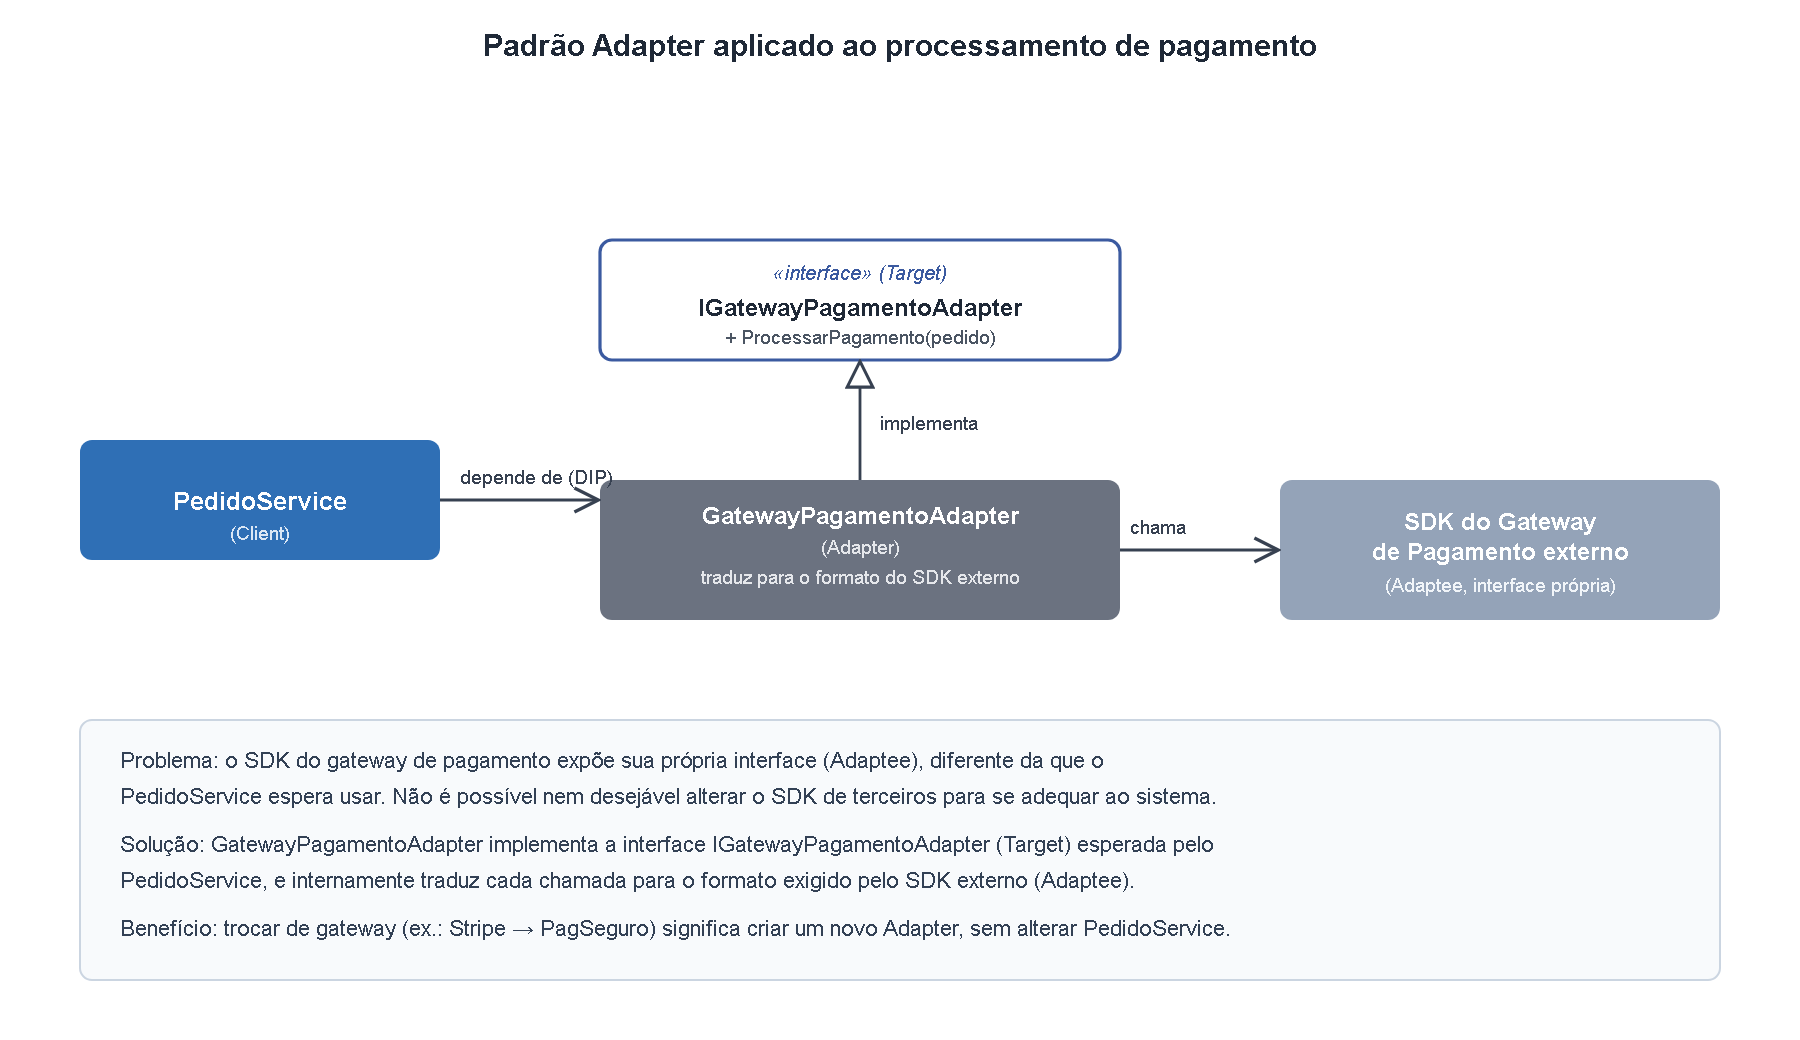
\includegraphics[width=0.85\textwidth]{padrao-adapter-pagamento.png}
\caption{Estrutura clássica do padrão Adapter (Target/Adapter/Adaptee) instanciada com as classes reais do caso de pagamento: \texttt{PedidoService} (Client) depende apenas de \texttt{IGatewayPagamentoAdapter} (Target); \texttt{GatewayPagamentoAdapter} implementa essa interface e traduz cada chamada para o SDK do gateway externo (Adaptee), cuja interface própria o sistema não controla.}
\label{fig:padrao-adapter}
\end{figure}

\textbf{Injeção de Dependência (via container do ASP.NET Core).} Problema: se cada Service instanciasse diretamente suas dependências concretas (o repositório do EF Core, o adapter HTTP do gateway de pagamento), o acoplamento entre camadas inviabilizaria tanto a testabilidade quanto a substituição de implementações discutidas no DIP. Solução adotada: registrar cada interface (\texttt{IPedidoRepository}, \texttt{IEstoqueService}, \texttt{IGatewayPagamentoAdapter} etc.) e sua implementação concreta correspondente no container de injeção de dependência nativo do ASP.NET Core, deixando que o framework resolva e injete as instâncias apropriadas nos construtores dos Services e Controllers em tempo de execução -- o construtor de \texttt{PedidoService} mostrado na seção de Princípios de projeto é exatamente o ponto de extensão que esse container preenche. Participantes: praticamente todos os componentes das camadas de Services, Repositories e External Adapters, mediados pelo container. Benefício obtido: as dependências entre camadas passam a ser configuradas externamente, e não codificadas dentro das classes, o que é a base técnica que sustenta tanto a testabilidade (substituir uma implementação real por um mock nos testes) quanto a substituição de tecnologia (trocar de gateway de pagamento ou de banco de dados) sem alterar código consumidor.

\textbf{Strategy.} Problema: diferentes gateways de pagamento (Stripe, PagSeguro, Pix) implementam o processamento de uma cobrança de formas distintas, e o sistema precisa poder trocar ou adicionar um gateway em produção sem recompilar ou alterar \texttt{PedidoService}. Solução adotada: cada gateway é encapsulado em uma implementação concreta de \texttt{IGatewayPagamentoAdapter}, e o \texttt{PedidoService} opera exclusivamente sobre essa abstração, recebendo a implementação ativa por injeção de dependência -- o mesmo mecanismo de configuração externa discutido na Injeção de Dependência acima. Participantes: \texttt{IGatewayPagamentoAdapter} (a estratégia comum), \texttt{GatewayPagamentoAdapter} e suas variantes por provedor (os algoritmos concretos), e \texttt{PedidoService} (o contexto que consome a estratégia sem conhecer qual está ativa). Benefício obtido: trocar o ``algoritmo'' de processamento de pagamento passa a ser uma decisão de configuração, não de código -- o mesmo caso já discutido como aplicação de OCP na seção anterior.

\textbf{Decorator.} Problema: um Item Personalizado nasce de um Produto Base ao qual o cliente vai adicionando um número variável de Ingredientes, cada um contribuindo com seu próprio preço e descrição ao resultado final -- exatamente o problema de explosão de subclasses discutido no exercício de Decorador da disciplina (lá, um carro com opcionais de navegação e cor; aqui, um lanche com ingredientes). Representar cada combinação possível de ingredientes como uma subclasse de \texttt{ProdutoBase} inviabilizaria o cardápio, já que o número de combinações cresce exponencialmente com o número de ingredientes disponíveis. Solução adotada: \texttt{ProdutoBase} e cada ingrediente adicionado implementam uma interface comum (\texttt{IItemPersonalizavel}, com \texttt{GetDescricao()} e \texttt{GetPreco()}); ao montar o pedido, cada \texttt{Ingrediente} selecionado envolve o item personalizado corrente em um \texttt{IngredienteDecorator}, que soma seu próprio preço ao preço acumulado e anexa sua descrição à do item envolvido, formando uma cadeia de decoradores equivalente ao objeto \texttt{ItemPersonalizado} final. Participantes: \texttt{IItemPersonalizavel} (o componente comum), \texttt{ProdutoBase} (o componente concreto que inicia a cadeia) e \texttt{IngredienteDecorator} (o decorador concreto, parametrizado pelo \texttt{Ingrediente} que representa). Benefício obtido: qualquer combinação de ingredientes é montada dinamicamente em tempo de execução, sem uma única subclasse nova; adicionar um ingrediente ao cardápio não exige tocar em \texttt{ProdutoBase} nem em nenhuma combinação já existente; e o preço é recalculado incrementalmente à medida que decoradores são empilhados -- o mesmo mecanismo que sustenta a atualização de preço em tempo real na interface do cliente, descrita no capítulo de Projeto de Interface do Usuário.

\begin{figure}[H]
\centering
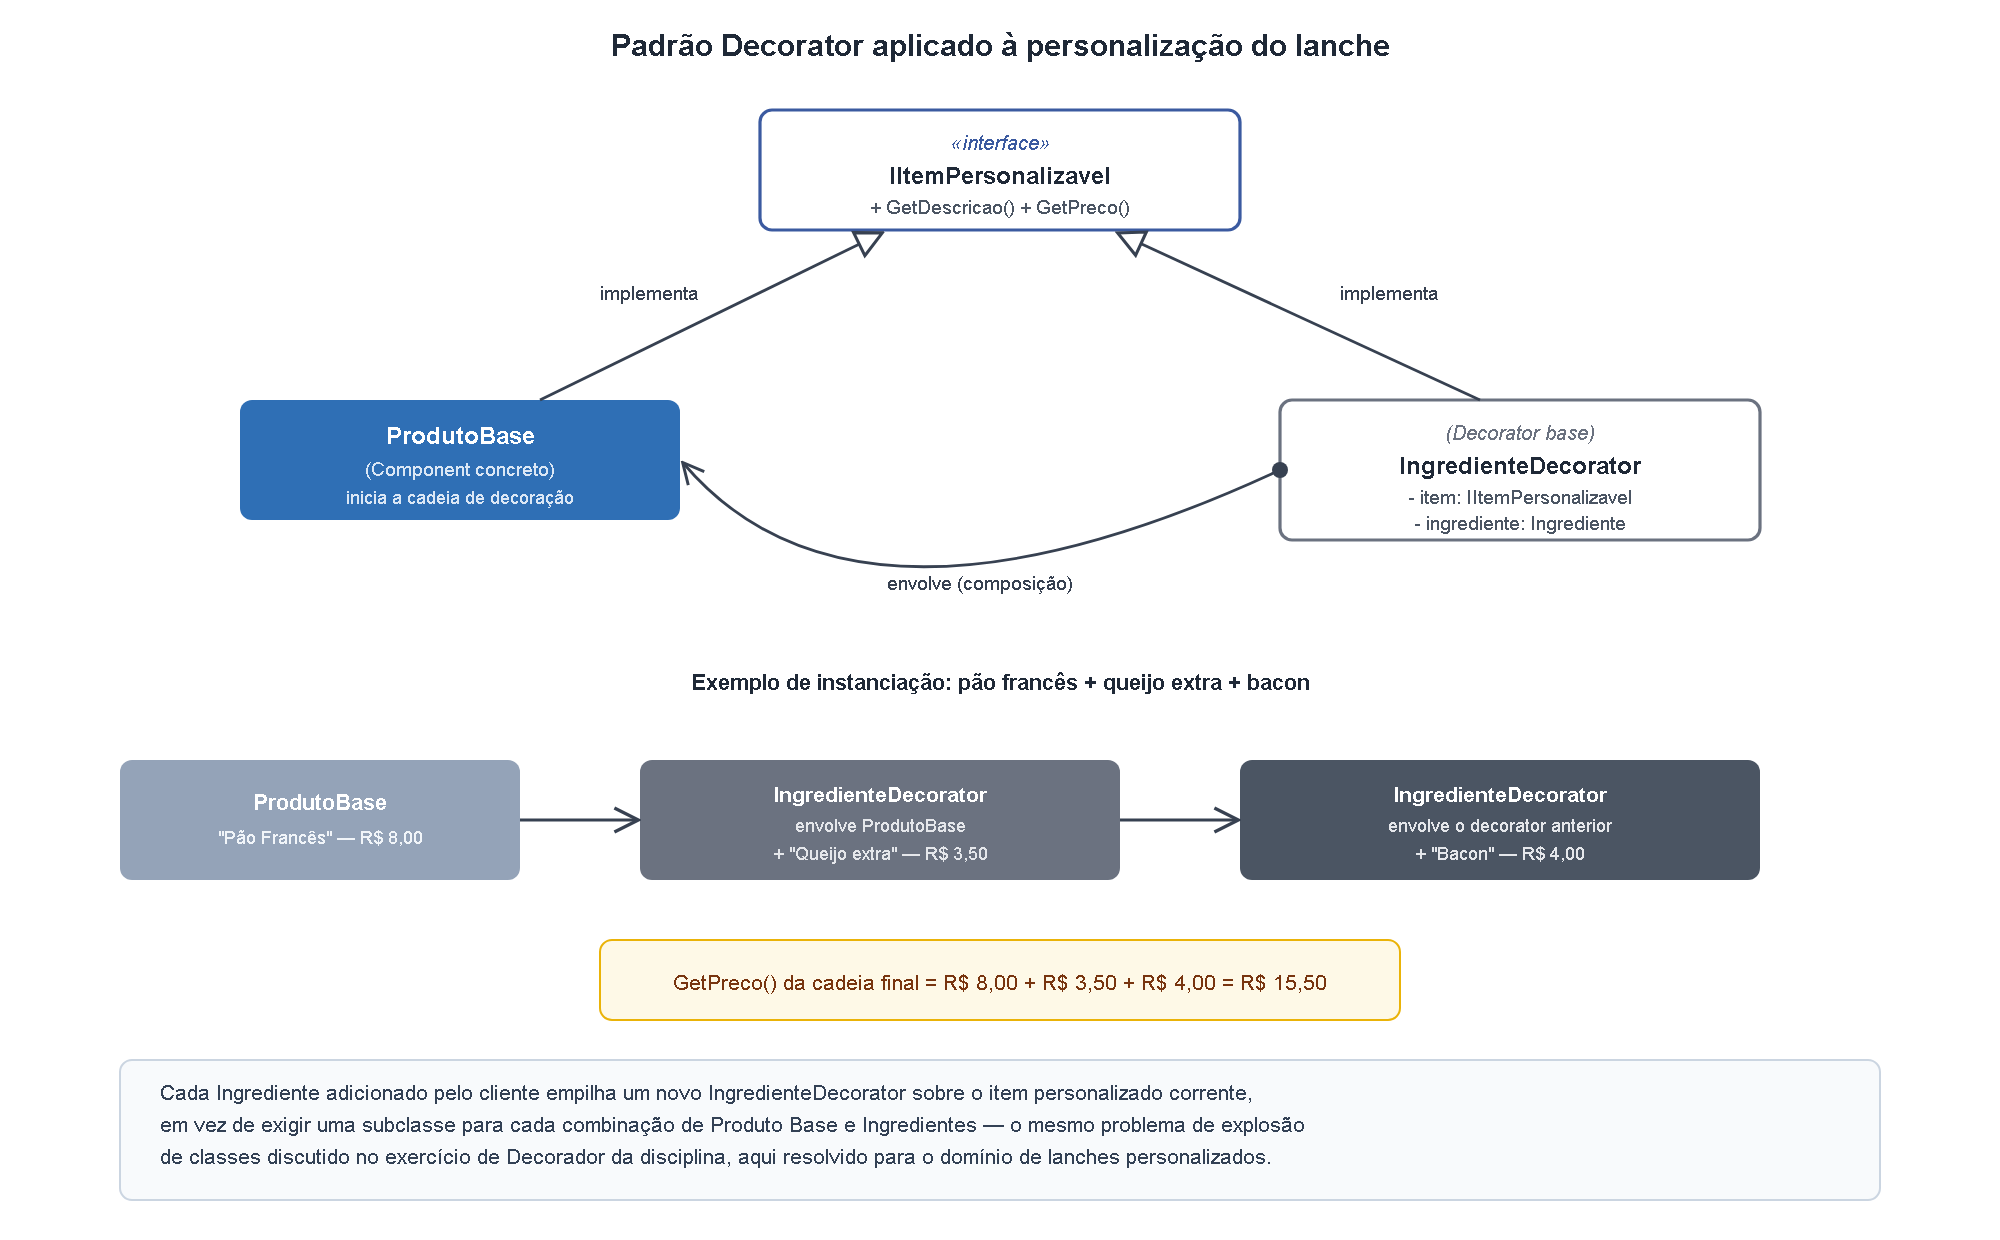
\includegraphics[width=0.85\textwidth]{padrao-decorator-personalizacao.png}
\caption{Estrutura do padrão Decorator (Component/ConcreteComponent/Decorator) aplicada à montagem de um Item Personalizado, com um exemplo concreto de instanciação (pão francês com queijo extra e bacon) mostrando como o preço se acumula a cada decorador empilhado.}
\label{fig:padrao-decorator}
\end{figure}

% ============================================================================
\chapter{Projeto de Interface do Usuário}
% ============================================================================

Este capítulo descreve os fluxos de interação com o Sistema Unespão para os dois perfis de usuário previstos no Minimundo: o Cliente, que monta e finaliza pedidos pelo totem físico da loja ou pelo aplicativo móvel, e o Atendente/Administrador da padaria, responsável pela gestão de catálogo e estoque. Diferente dos capítulos de arquitetura, aqui o foco não é a estrutura interna do software, mas a experiência de quem está usando o sistema em cada um desses papéis.

\section{Artefatos de interface}

O projeto de interface do Sistema Unespão é descrito neste capítulo por meio de diagramas de atividade e de uma especificação estrutural detalhada de cada tela, cobrindo os dois perfis de usuário: Cliente e Atendente/Administrador. Essa especificação registra, para cada etapa do fluxo, o que a tela exibe, quais ações o usuário pode tomar e para onde cada ação leva -- o nível de detalhe necessário para que a equipe de desenvolvimento implemente as telas sem ambiguidade, independentemente da ferramenta de prototipação visual usada para desenhá-las (Figma ou equivalente).

As decisões estruturais do fluxo -- a ordem das etapas, o que cada uma exige do usuário e, em particular, como funciona a autenticação num dispositivo compartilhado -- foram discutidas e fixadas pelo PO, e são o conteúdo deste capítulo.

\section{Canais de interação do Cliente}

O cliente acessa o sistema por um destes dois canais, que compartilham a mesma lógica de negócio no backend (API Unespão) e diferem principalmente na forma de entrada:

\begin{itemize}
    \item \textbf{Totem físico}, instalado na loja, pensado para o cliente que já está presencialmente na padaria e decide o pedido ali mesmo. É um dispositivo compartilhado entre vários clientes ao longo do dia.
    \item \textbf{Aplicativo móvel}, no celular do próprio cliente, usado tanto para pedir remotamente quanto para complementar a experiência do totem -- por exemplo, quando o cliente já chega com uma conta autenticada.
\end{itemize}

Os passos do pedido (escolha do produto, personalização, pagamento) são conceitualmente os mesmos nos dois canais. A diferença que importa do ponto de vista de projeto de interface está na etapa de autenticação, tratada separadamente mais adiante.

\section{Fluxo principal de interação do cliente}

O fluxo de ponta a ponta, do início do pedido até a etapa posterior de avaliação, segue as seguintes etapas:

\begin{enumerate}
    \item \textbf{Identificação no canal.} No aplicativo, o cliente autentica normalmente -- contas de clientes recorrentes têm histórico de pedidos associado, conforme o Minimundo. No totem, a identificação segue a decisão de projeto detalhada na próxima seção: QR code vinculando a sessão do app, ou pedido anônimo com vínculo posterior.
    \item \textbf{Escolha do produto base.} O cliente seleciona o item que servirá de ponto de partida para a personalização, por exemplo um tipo de pão ou uma base de salada, dentre os produtos disponíveis em estoque.
    \item \textbf{Adição de ingredientes com atualização incremental do preço.} A cada ingrediente adicionado ou removido, o valor do item é recalculado e exibido imediatamente, sem que o cliente precise avançar de tela para saber o custo da personalização. Essa atualização incremental existe porque o preço final de um Item Personalizado só é conhecido depois da composição completa de Ingredientes, e faz sentido que o cliente acompanhe esse custo enquanto ainda está decidindo: evita surpresa na etapa de revisão e reduz a chance de abandono do pedido.
    \item \textbf{Revisão do pedido.} Antes de seguir para o pagamento, o cliente vê o resumo dos itens personalizados escolhidos, com a possibilidade de cancelar ou editar qualquer item. Este ponto está alinhado ao requisito funcional já definido pelo PO de permitir alteração do pedido antes da confirmação do pagamento.
\end{enumerate}

A Figura~\ref{fig:tela-escolha-base-resumo} ilustra a estrutura de tela adotada para as etapas 2 e 3: à esquerda, o passo de escolha da base do lanche, com cada Produto Base listado junto de suas informações nutricionais, tempo de preparo e preço, e a base já selecionada destacada visualmente; à direita, um painel de resumo em tempo real que acompanha o cliente por toda a montagem do item, recalculando o preço a cada ingrediente adicionado, exatamente o comportamento descrito na etapa 3.

\begin{figure}[H]
\centering
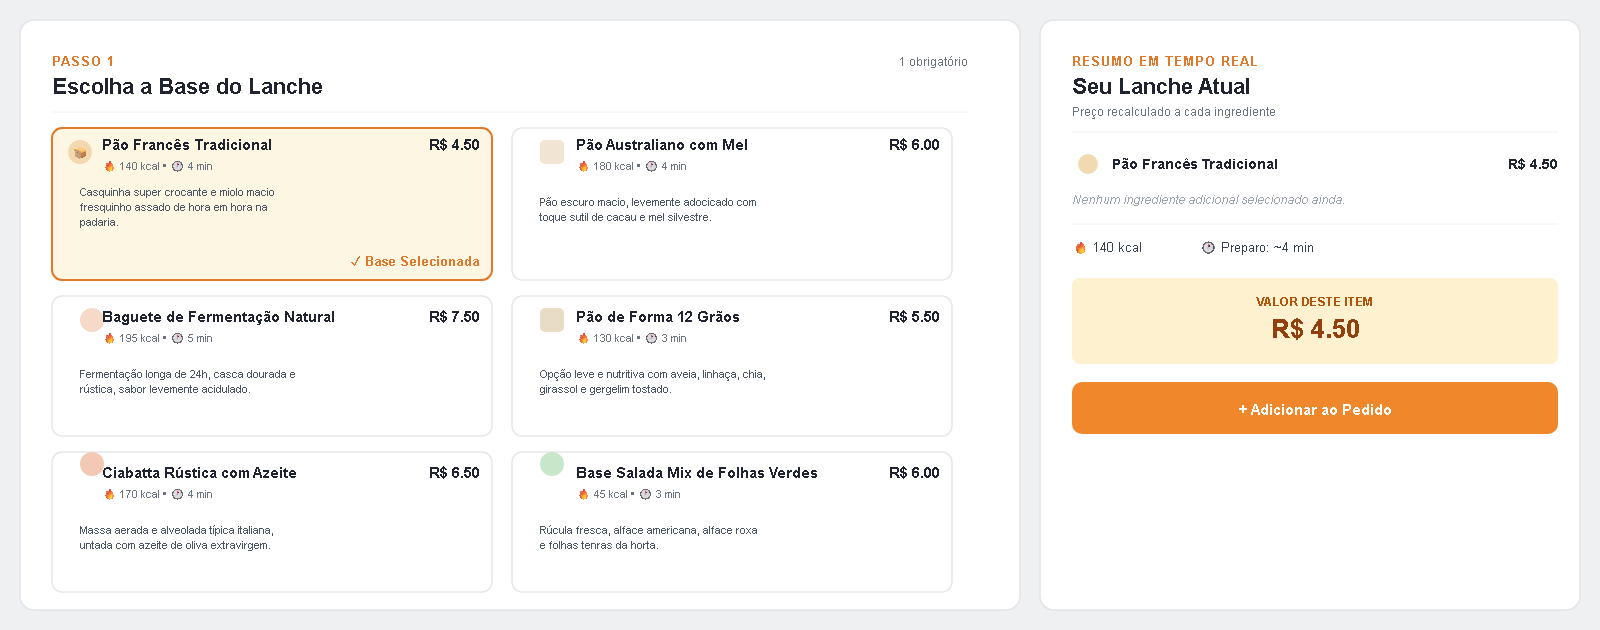
\includegraphics[width=0.95\textwidth]{tela-escolha-base-resumo.png}
\caption{Passo 1 do fluxo (escolha da base), com o painel de resumo em tempo real à direita: o preço do item é recalculado a cada seleção, antes mesmo de o cliente começar a adicionar ingredientes.}
\label{fig:tela-escolha-base-resumo}
\end{figure}

\begin{enumerate}
    \setcounter{enumi}{4}
    \item \textbf{Pagamento.} O pedido é encaminhado ao Gateway de Pagamento via API Unespão, nunca diretamente do frontend, como descrito na arquitetura, e o cliente acompanha o status da transação.
    \item \textbf{Confirmação.} Com o pagamento aprovado, o pedido é registrado e o cliente recebe a confirmação, encerrando o ciclo ativo de compra.
    \item \textbf{Avaliação do prato (momento posterior).} Depois de retirar o pedido, o cliente pode registrar uma Avaliação de Prato: nota e comentário sobre o Item Personalizado consumido.
    \item \textbf{Sugestões personalizadas em pedidos futuros.} Em pedidos seguintes, o sistema usa o Histórico de Pedidos e as avaliações anteriores para propor combinações que o cliente tende a gostar, reduzindo o número de decisões que ele precisa tomar do zero a cada visita.
\end{enumerate}

O diagrama de atividade a seguir representa essas oito etapas, já incluindo a bifurcação de identificação no totem (QR code vs. pedido anônimo) detalhada na seção seguinte:

\begin{figure}[H]
\centering
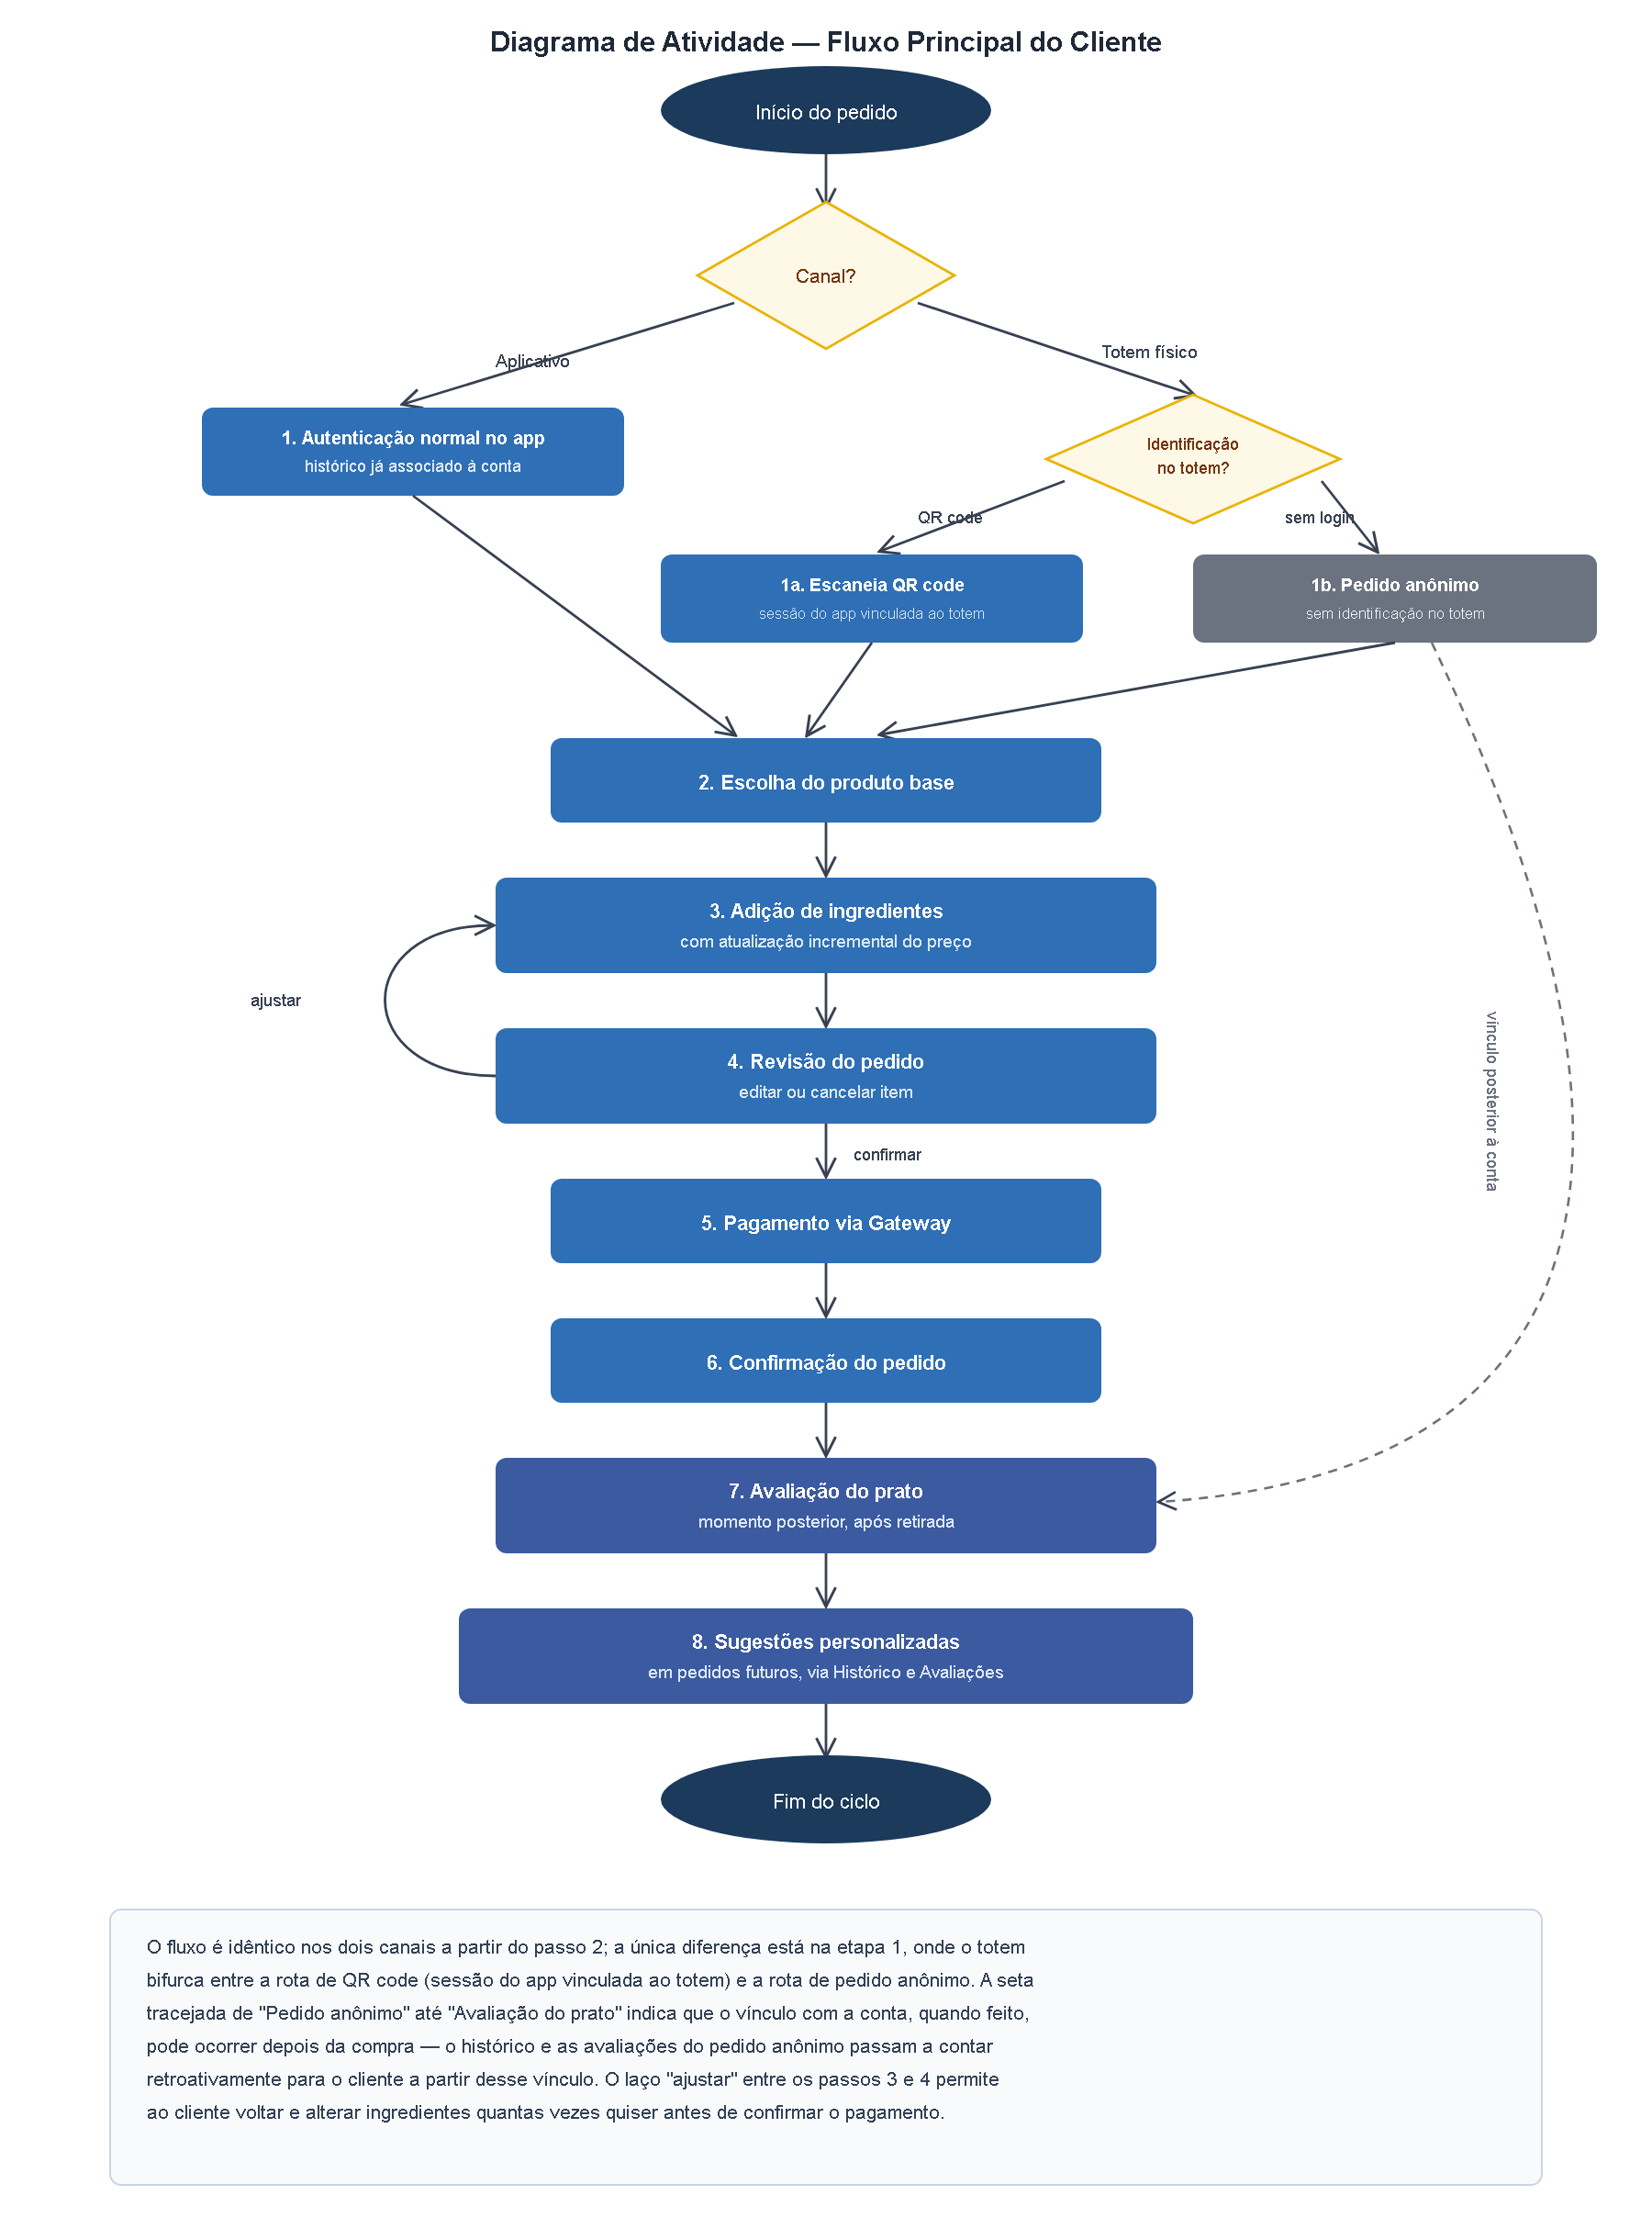
\includegraphics[width=0.75\textwidth]{atividade-fluxo-cliente.png}
\caption{Diagrama de atividade das oito etapas do fluxo do Cliente, da identificação no canal até a geração de sugestões personalizadas em pedidos futuros.}
\label{fig:atividade-fluxo-cliente}
\end{figure}

O fluxo é o mesmo nos dois canais a partir do passo 2; a diferença está inteiramente na etapa 1, onde o totem bifurca entre a rota de QR code e a rota anônima. A seta pontilhada de ``pedido anônimo'' até a etapa de avaliação indica que esse vínculo com a conta, quando feito, pode ocorrer depois da compra, permitindo que o histórico e as avaliações do pedido anônimo passem a contar retroativamente para o cliente.

\section{Decisão de projeto: autenticação no totem físico}

Um ponto que exigiu decisão explícita do PO foi como identificar o cliente no totem, já que esse dispositivo é compartilhado por múltiplos clientes ao longo do dia, diferente do celular no app, que é de uso pessoal.

Duas alternativas foram descartadas antes de chegar à decisão final. A primeira era exigir um fluxo completo de OAuth 2.0, o mesmo usado pelo Serviço de Autenticação do Google já presente na arquitetura, diretamente no totem. Isso obrigaria o cliente a digitar credenciais num teclado público, o que é ruim tanto em usabilidade (login lento, digitação incômoda numa tela touch) quanto em segurança, pela exposição da senha ou do token de sessão num equipamento compartilhado: se a sessão de um cliente não fosse encerrada corretamente, o próximo cliente poderia herdar o carrinho ou o histórico de quem usou o totem antes dele. A segunda alternativa cogitada foi autenticar apenas por CPF, descartada por não constituir autenticação forte (qualquer pessoa que soubesse o CPF de outra poderia se passar por ela) e por não ter respaldo em nenhuma das fontes do projeto.

A solução adotada combina duas rotas, e o cliente escolhe entre elas no início do fluxo do totem:

\begin{itemize}
    \item \textbf{QR code vinculado à sessão do app.} O cliente abre o aplicativo no próprio celular, já autenticado ali, e usa essa sessão para gerar um QR code que o totem lê. A partir daí, o totem apenas associa o pedido em andamento à conta já logada no celular: nenhuma credencial é digitada no dispositivo público, e a sessão fica atrelada ao aparelho do cliente, não ao totem.
    \item \textbf{Pedido anônimo, com vínculo posterior.} Se o cliente preferir não usar o app naquele momento, o totem permite montar e pagar o pedido sem identificação alguma. Depois, ele pode vincular esse pedido à sua conta, por exemplo abrindo o app e associando o comprovante ou pedido recente, passando a contar para o Histórico de Pedidos e para as Sugestões Personalizadas.
\end{itemize}

Essa decisão evita reintroduzir no totem o mesmo risco que motivou o descarte do OAuth completo, a sessão cruzada entre clientes num equipamento compartilhado, e ainda preserva o benefício de histórico e recomendação para quem quiser se identificar. O custo é aceitar que uma parcela dos pedidos feitos no totem fique anônima, sem entrar no cálculo de Sugestões Personalizadas, a menos que o cliente faça questão de vincular depois.

O diagrama a seguir isola essa bifurcação, detalhando o que cada rota exige do dispositivo e da conta:

\begin{figure}[H]
\centering
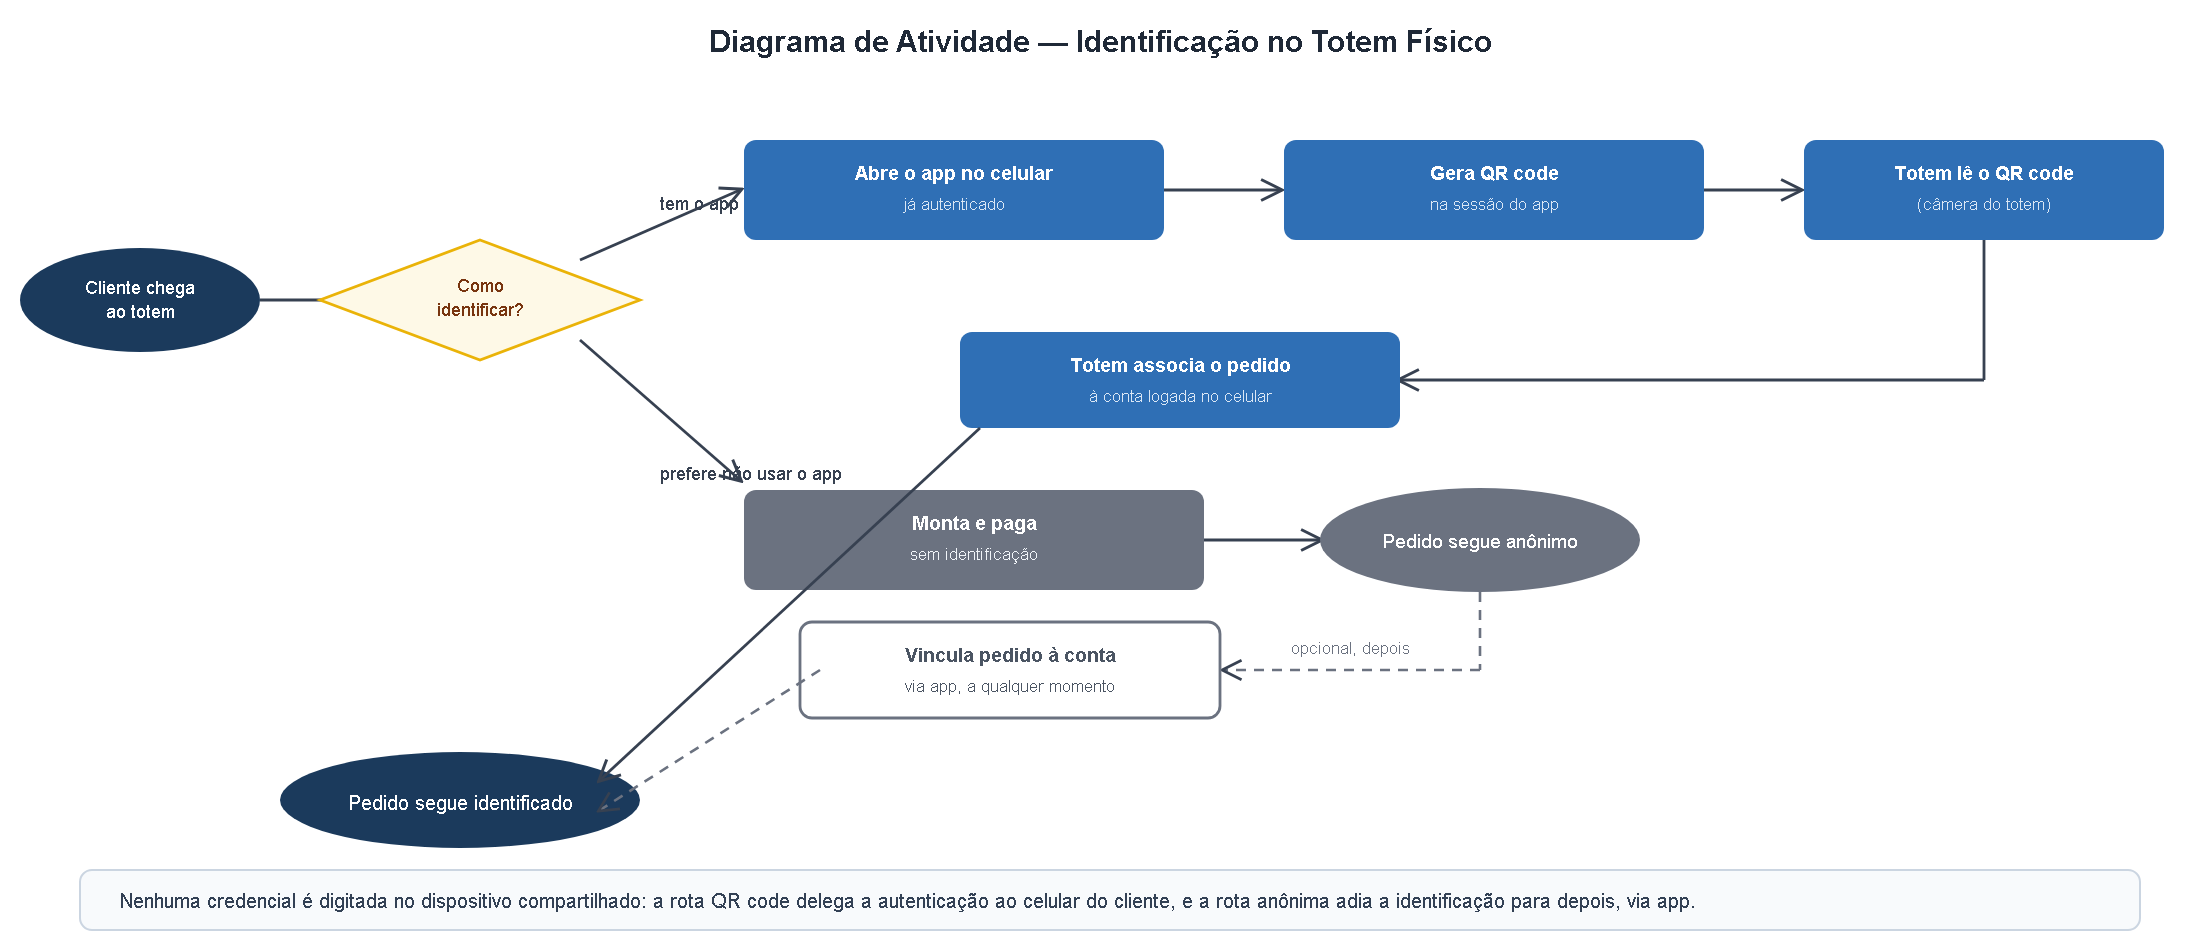
\includegraphics[width=0.95\textwidth]{atividade-autenticacao-totem.png}
\caption{As duas rotas de identificação no totem: QR code vinculado à sessão do app, ou pedido anônimo com vínculo posterior à conta.}
\label{fig:atividade-autenticacao-totem}
\end{figure}

\section{Interface do Atendente/Administrador}

Além do Cliente, o sistema prevê um segundo perfil de usuário: o Atendente/Administrador da padaria, responsável pela gestão de catálogo (produtos base e ingredientes) e de estoque. Esse é um perfil de uso interno, operado por quem trabalha na padaria, e não pelo cliente final -- por isso seu canal de acesso é tratado separadamente do totem e do aplicativo do cliente.

O Atendente/Administrador acessa um painel administrativo web, servido pelo mesmo SPA React que atende o Cliente no totem e no navegador, mas com uma rota e um conjunto de telas próprios, visíveis apenas após autenticação com credenciais de funcionário. Esse painel é deliberadamente mais simples do que a experiência do Cliente: não há personalização de pedido nem etapas sequenciais a percorrer, apenas duas telas de gestão (Catálogo e Estoque) acessíveis a qualquer momento pelo menu principal.

A interface desse perfil é estruturalmente mais simples que a do Cliente: não envolve personalização de pedido, atualização incremental de preço, pagamento ou avaliação de prato. Suas operações centrais são de CRUD (criação, leitura, atualização e remoção) sobre duas famílias de dados:

\begin{itemize}
    \item \textbf{Catálogo.} Cadastro e manutenção dos Produtos Base (por exemplo, tipos de pão ou bases de salada) e dos Ingredientes disponíveis para personalização, incluindo os dados que o Cliente vê no momento de montar seu pedido, como nome, descrição e preço unitário de cada ingrediente.
    \item \textbf{Estoque.} Atualização das quantidades disponíveis de cada Produto Base e Ingrediente, refletindo o que efetivamente pode ser oferecido ao Cliente no totem e no aplicativo. É essa informação de estoque que impede, por exemplo, que um cliente monte um pedido com um ingrediente esgotado.
\end{itemize}

Essas operações de catálogo e estoque feitas pelo Atendente/Administrador alimentam diretamente os dados que o Cliente consome nos passos 2 e 3 do fluxo principal descrito anteriormente: a lista de produtos disponíveis e o preço de cada ingrediente vêm dessa gestão interna. Por isso, embora os dois perfis usem canais e telas distintas, suas interfaces não são independentes -- são duas pontas do mesmo ciclo de dados do sistema.

% ============================================================================
\chapter{Especificação e Estratégia de Testes}
% ============================================================================

O Sistema Unespão concentra praticamente toda a lógica de negócio na API Unespão (.NET 8 / ASP.NET Core), enquanto o Web App/Totem funciona como uma camada de apresentação relativamente fina, que consome essa API via HTTPS/JSON. Por isso a estratégia de testes da equipe se concentra no backend: é ali que vivem as regras que decidem se um pedido pode ser fechado, se há insumo suficiente no estoque e como um item personalizado tem seu preço calculado. Este capítulo descreve os níveis de teste adotados, os critérios usados para selecionar o que testar e as ferramentas do ecossistema .NET que sustentam essa estratégia.

Um ponto de partida importante é a própria arquitetura em camadas descrita no capítulo de Arquitetura (Controllers $\rightarrow$ Services $\rightarrow$ Repositories/External Adapters $\rightarrow$ Domain Models, com fluxo de dependência unidirecional). Como os Services dependem de abstrações -- \texttt{IPedidoRepository}, \texttt{IEstoqueRepository}, \texttt{IGatewayPagamentoAdapter}, entre outras -- e não de classes concretas, a própria organização do código já favorece testes isolados: basta substituir a implementação real por um dublê de teste sem tocar em nenhuma linha da classe testada.

\section{Planejamento e níveis de teste}

Adotamos três níveis de teste, cada um respondendo a uma pergunta diferente sobre o sistema.

Os \textbf{testes de unidade} verificam se uma classe de negócio se comporta corretamente quando isolada de tudo à sua volta. O alvo principal aqui são os Services (\texttt{PedidoService}, \texttt{EstoqueService}, \texttt{ProdutoService} etc.) e os Domain Models com lógica própria, como \texttt{ItemPersonalizado}. A pergunta que esse nível responde é: esta unidade de código faz o que deveria, dado um conjunto controlado de entradas?

Já os \textbf{testes de integração} verificam se as peças que se comunicam entre si -- no nosso caso, principalmente a API Unespão e o banco PostgreSQL via Entity Framework Core/Npgsql -- realmente conversam corretamente quando combinadas. Aqui a pergunta muda: não é mais ``a lógica está certa isoladamente'', e sim se o Repository gera o SQL certo, se o mapeamento do EF Core está coerente com o schema e se a operação persiste e recupera os dados como esperado.

O terceiro nível, testes de sistema, valida o fluxo ponta a ponta através da interface real, via totem/app: o cliente autentica, monta um item personalizado, paga e recebe a confirmação, exatamente como especificado no capítulo de Interface do Usuário. Esses testes rodam sobre o SPA React já renderizado num navegador automatizado, exercitando a pilha completa (interface, API, banco de dados e o gateway de pagamento, este último substituído por um ambiente de sandbox do provedor) e servem sobretudo para pegar problemas de integração entre camadas que nenhum teste isolado revela, como uma tela que não reflete corretamente um erro de pagamento devolvido pela API.

\begin{figure}[H]
\centering

\includegraphics[width=0.75\textwidth]{piramide-testes.png}
\caption{A pirâmide de testes é um modelo conceitual conhecido da literatura de teste de software (não um conteúdo específico dos slides da disciplina), usado aqui para situar visualmente os três níveis adotados: muitos testes de unidade rápidos na base, um número intermediário de testes de integração e, no topo, um conjunto mais enxuto de testes de sistema ponta a ponta.}
\label{fig:piramide-testes}
\end{figure}

A prioridade de testes segue a mesma lógica dos objetivos de qualidade definidos na Introdução: como ``Confiabilidade da informação de estoque'' e ``Segurança dos dados e transações do cliente'' foram marcados como prioridade Alta, \texttt{EstoqueService} e o fluxo de pagamento (\texttt{PedidoService} + \texttt{IGatewayPagamentoAdapter}) recebem mais atenção de teste do que, por exemplo, \texttt{SugestaoPersonalizadaService}, cujo objetivo de qualidade associado (``Relevância das sugestões personalizadas'') tem prioridade Média.

\section{Testes de unidade}

A ideia central desta seção é a mesma trabalhada no exercício de testes de unidade da disciplina (\texttt{ProcessadorVendas} com e sem \texttt{Mockito}), só que transposta para o ecossistema real do projeto: em vez de JUnit e Mockito sobre um \texttt{ProcessadorVendas} de exemplo, usamos \textbf{xUnit} como framework de teste e \textbf{Moq} como biblioteca de mocks sobre as classes reais do Sistema Unespão, escritas em C\#.

\subsection*{PedidoService com IPedidoRepository mockado}

O \texttt{PedidoService} é o candidato mais natural para essa técnica, porque o próprio documento de arquitetura já cita esse par como exemplo de LSP: \texttt{PedidoRepository} (PostgreSQL real) e \texttt{MockPedidoRepository}/dublê de teste devem ser intercambiáveis do ponto de vista do \texttt{PedidoService}. Um teste sem mock, usando uma implementação em memória do repositório, ficaria assim:

\begin{lstlisting}[language=csharp, caption={Teste sem mock, com repositório e gateway em memória.}]
public class PedidoServiceSemMockTests
{
    [Fact]
    public void FinalizarPedido_ComEstoqueSuficiente_RetornaSucesso()
    {
        var repositorioEmMemoria = new PedidoRepositoryEmMemoria();
        var estoqueService = new EstoqueServiceEmMemoria();
        var gatewayFake = new GatewayPagamentoSempreAprova();

        var service = new PedidoService(repositorioEmMemoria, estoqueService, gatewayFake);

        var resultado = service.FinalizarPedido(pedidoId: 1);

        Assert.Equal(StatusPedido.Confirmado, resultado.Status);
    }
}
\end{lstlisting}

Essa abordagem funciona, mas exige manter classes auxiliares ``de mentira'' (\texttt{PedidoRepositoryEmMemoria}, \texttt{GatewayPagamentoSempreAprova}) só para viabilizar o teste, e qualquer mudança de comportamento nelas pode mascarar um defeito real. A abordagem com Moq resolve isso criando o dublê dinamicamente, a partir da própria interface:

\begin{lstlisting}[language=csharp, caption={Testes com Moq, cobrindo pagamento aprovado e pagamento recusado.}]
public class PedidoServiceComMockTests
{
    private readonly Mock<IPedidoRepository> _repositorioMock;
    private readonly Mock<IEstoqueService> _estoqueMock;
    private readonly Mock<IGatewayPagamentoAdapter> _gatewayMock;
    private readonly PedidoService _service;

    public PedidoServiceComMockTests()
    {
        _repositorioMock = new Mock<IPedidoRepository>();
        _estoqueMock = new Mock<IEstoqueService>();
        _gatewayMock = new Mock<IGatewayPagamentoAdapter>();
        _service = new PedidoService(_repositorioMock.Object, _estoqueMock.Object, _gatewayMock.Object);
    }

    [Fact]
    public void FinalizarPedido_PagamentoAprovado_AtualizaStatusParaConfirmado()
    {
        var pedido = new Pedido { Id = 1, Status = StatusPedido.Aberto, ValorTotal = 35.90m };
        _repositorioMock.Setup(r => r.GetById(1)).Returns(pedido);
        _estoqueMock.Setup(e => e.HaSaldoSuficiente(pedido)).Returns(true);
        _gatewayMock.Setup(g => g.Cobrar(It.IsAny<string>(), pedido.ValorTotal)).Returns(true);

        var resultado = _service.FinalizarPedido(1);

        Assert.Equal(StatusPedido.Confirmado, resultado.Status);
        _repositorioMock.Verify(r => r.Update(It.Is<Pedido>(p => p.Status == StatusPedido.Confirmado)), Times.Once);
    }

    [Fact]
    public void FinalizarPedido_PagamentoRecusado_MantemPedidoAbertoENaoDaBaixaNoEstoque()
    {
        var pedido = new Pedido { Id = 2, Status = StatusPedido.Aberto, ValorTotal = 20.00m };
        _repositorioMock.Setup(r => r.GetById(2)).Returns(pedido);
        _estoqueMock.Setup(e => e.HaSaldoSuficiente(pedido)).Returns(true);
        _gatewayMock.Setup(g => g.Cobrar(It.IsAny<string>(), pedido.ValorTotal)).Returns(false);

        var resultado = _service.FinalizarPedido(2);

        Assert.Equal(StatusPedido.PagamentoRecusado, resultado.Status);
        _estoqueMock.Verify(e => e.DarBaixa(It.IsAny<Pedido>()), Times.Never);
    }
}
\end{lstlisting}

O segundo teste é particularmente útil porque exercita um cenário que seria trabalhoso de forçar com um gateway real (uma recusa de pagamento) e verifica uma consequência que importa para a confiabilidade do estoque: se o pagamento falha, a baixa de insumos não pode acontecer. Isolar o \texttt{PedidoService} do gateway de pagamento real também evita que a suíte de testes dependa de rede, de credenciais ou da disponibilidade de um serviço externo, o que tornaria os testes lentos e instáveis.

\subsection*{EstoqueService: baixa de insumos}

O \texttt{EstoqueService} concentra uma regra sensível: dar baixa nos insumos (produtos base e ingredientes) associados aos itens de um pedido, sem deixar o saldo ficar negativo. Aqui a atenção recai sobre os casos de borda: saldo exato, saldo insuficiente, item com quantidade zero.

\begin{lstlisting}[language=csharp, caption={Testes de \texttt{EstoqueService} cobrindo saldo exato e saldo insuficiente.}]
[Fact]
public void DarBaixa_ComSaldoExato_ZeraEstoqueSemErro()
{
    var estoqueMock = new Mock<IEstoqueRepository>();
    estoqueMock.Setup(r => r.GetByIngredienteId(10)).Returns(new Estoque { QuantidadeDisponivel = 2 });

    var service = new EstoqueService(estoqueMock.Object);
    service.DarBaixa(ingredienteId: 10, quantidade: 2);

    estoqueMock.Verify(r => r.Update(It.Is<Estoque>(e => e.QuantidadeDisponivel == 0)), Times.Once);
}

[Fact]
public void DarBaixa_ComSaldoInsuficiente_LancaExcecaoENaoAtualizaEstoque()
{
    var estoqueMock = new Mock<IEstoqueRepository>();
    estoqueMock.Setup(r => r.GetByIngredienteId(10)).Returns(new Estoque { QuantidadeDisponivel = 1 });

    var service = new EstoqueService(estoqueMock.Object);

    Assert.Throws<EstoqueInsuficienteException>(() => service.DarBaixa(ingredienteId: 10, quantidade: 2));
    estoqueMock.Verify(r => r.Update(It.IsAny<Estoque>()), Times.Never);
}
\end{lstlisting}

Na prática, o segundo caso é o mais importante dos dois: ele garante que uma tentativa de baixa acima do saldo disponível não corrompe silenciosamente o estoque, algo diretamente ligado ao objetivo de qualidade de confiabilidade da informação de estoque discutido na Introdução.

\subsection*{Cálculo de preço de um ItemPersonalizado}

Diferente dos exemplos anteriores, o cálculo de preço de um \texttt{ItemPersonalizado} é um caso de teste de unidade sem qualquer dependência externa a isolar: é lógica pura sobre os dados do próprio objeto (preço base do produto mais a soma dos preços adicionais dos ingredientes selecionados). Isso o torna um bom exemplo de teste ``sem mock'', no espírito do primeiro teste do exercício de referência da disciplina:

\begin{lstlisting}[language=csharp, caption={Teste puro (sem mock) do cálculo de preço de um item personalizado.}]
public class ItemPersonalizadoTests
{
    [Fact]
    public void CalcularPrecoTotal_ComIngredientesAdicionais_SomaPrecoBaseEAdicionais()
    {
        var produtoBase = new ProdutoBase { Nome = "Pao Frances", PrecoBase = 8.00m };
        var ingredientes = new List<Ingrediente>
        {
            new Ingrediente { Nome = "Queijo extra", PrecoAdicional = 3.50m },
            new Ingrediente { Nome = "Bacon", PrecoAdicional = 4.00m }
        };

        var item = new ItemPersonalizado(produtoBase, ingredientes);

        Assert.Equal(15.50m, item.PrecoTotal);
    }

    [Fact]
    public void CalcularPrecoTotal_SemIngredientesAdicionais_IgualAoPrecoBase()
    {
        var produtoBase = new ProdutoBase { Nome = "Pao Frances", PrecoBase = 8.00m };
        var item = new ItemPersonalizado(produtoBase, new List<Ingrediente>());

        Assert.Equal(8.00m, item.PrecoTotal);
    }
}
\end{lstlisting}

\subsection*{Autenticação via Google OAuth 2.0}

A autenticação do cliente no aplicativo, que o \texttt{ClienteService} resolve integrando o Google OAuth 2.0 através do \texttt{IGoogleAuthAdapter}, é diretamente ligada ao objetivo de qualidade de segurança de prioridade Alta e por isso recebe o mesmo tratamento de teste dado a \texttt{PedidoService} e \texttt{EstoqueService}: o teste isola o \texttt{ClienteService} do provedor externo, mockando \texttt{IGoogleAuthAdapter}, e cobre tanto o caminho de sucesso quanto o de falha.

\begin{lstlisting}[language=csharp, caption={Testes de \texttt{ClienteService} cobrindo token do Google válido e inválido.}]
public class ClienteServiceAutenticacaoComMockTests
{
    private readonly Mock<IGoogleAuthAdapter> _googleAuthMock;
    private readonly Mock<IClienteRepository> _clienteRepositoryMock;
    private readonly ClienteService _service;

    public ClienteServiceAutenticacaoComMockTests()
    {
        _googleAuthMock = new Mock<IGoogleAuthAdapter>();
        _clienteRepositoryMock = new Mock<IClienteRepository>();
        _service = new ClienteService(_googleAuthMock.Object, _clienteRepositoryMock.Object);
    }

    [Fact]
    public void Autenticar_TokenGoogleValido_RetornaClienteAutenticado()
    {
        var tokenGoogle = "token-valido-simulado";
        _googleAuthMock.Setup(g => g.ValidarToken(tokenGoogle))
            .Returns(new GoogleUserInfo { Email = "cliente@example.com", Nome = "Cliente Teste" });
        _clienteRepositoryMock.Setup(r => r.GetByEmail("cliente@example.com"))
            .Returns(new Cliente { Id = 1, Email = "cliente@example.com" });

        var resultado = _service.Autenticar(tokenGoogle);

        Assert.True(resultado.Sucesso);
        Assert.Equal(1, resultado.ClienteId);
    }

    [Fact]
    public void Autenticar_TokenGoogleInvalido_RetornaFalhaSemConsultarRepositorio()
    {
        var tokenInvalido = "token-invalido-simulado";
        _googleAuthMock.Setup(g => g.ValidarToken(tokenInvalido)).Returns((GoogleUserInfo)null);

        var resultado = _service.Autenticar(tokenInvalido);

        Assert.False(resultado.Sucesso);
        _clienteRepositoryMock.Verify(r => r.GetByEmail(It.IsAny<string>()), Times.Never);
    }
}
\end{lstlisting}

O segundo teste importa tanto quanto o primeiro: um token rejeitado pelo Google nunca deve chegar a consultar ou criar um registro de cliente, o que evita que uma falha de autenticação vaze para outras camadas do sistema.

\subsection*{Edição e cancelamento de item antes da confirmação do pagamento}

Editar ou remover um item de um pedido ainda aberto é uma funcionalidade de prioridade Alta, por afetar diretamente o valor total cobrado e o cálculo de baixa de estoque. O teste de unidade correspondente cobre tanto a edição bem-sucedida quanto a tentativa de alterar um pedido que já foi confirmado, o que deve ser bloqueado:

\begin{lstlisting}[language=csharp, caption={Testes de \texttt{PedidoService} cobrindo remoção de item em pedido aberto e em pedido já confirmado.}]
public class PedidoServiceEdicaoItemTests
{
    [Fact]
    public void RemoverItem_PedidoAindaAberto_AtualizaValorTotalERemoveItem()
    {
        var repositorioMock = new Mock<IPedidoRepository>();
        var pedido = new Pedido { Id = 3, Status = StatusPedido.Aberto, ValorTotal = 23.50m };
        pedido.Itens.Add(new ItemPedido { Id = 100, PrecoTotal = 8.00m });
        pedido.Itens.Add(new ItemPedido { Id = 101, PrecoTotal = 15.50m });
        repositorioMock.Setup(r => r.GetById(3)).Returns(pedido);

        var service = new PedidoService(repositorioMock.Object, Mock.Of<IEstoqueService>(), Mock.Of<IGatewayPagamentoAdapter>());
        var resultado = service.RemoverItem(pedidoId: 3, itemId: 100);

        Assert.Equal(15.50m, resultado.ValorTotal);
        Assert.DoesNotContain(resultado.Itens, i => i.Id == 100);
    }

    [Fact]
    public void RemoverItem_PedidoJaConfirmado_LancaExcecaoENaoAlteraPedido()
    {
        var repositorioMock = new Mock<IPedidoRepository>();
        var pedido = new Pedido { Id = 4, Status = StatusPedido.Confirmado, ValorTotal = 12.00m };
        pedido.Itens.Add(new ItemPedido { Id = 200, PrecoTotal = 12.00m });
        repositorioMock.Setup(r => r.GetById(4)).Returns(pedido);

        var service = new PedidoService(repositorioMock.Object, Mock.Of<IEstoqueService>(), Mock.Of<IGatewayPagamentoAdapter>());

        Assert.Throws<PedidoJaConfirmadoException>(() => service.RemoverItem(pedidoId: 4, itemId: 200));
        repositorioMock.Verify(r => r.Update(It.IsAny<Pedido>()), Times.Never);
    }
}
\end{lstlisting}

O segundo teste é o que protege a regra de negócio: uma vez que o pagamento foi confirmado, o pedido já gerou baixa de estoque e não pode mais ser alterado sem descompassar o saldo, então qualquer tentativa de edição nesse estágio precisa ser rejeitada antes de tocar o repositório.

\subsection*{Critério de seleção das unidades testadas}

Não pretendemos cobrir cada classe do sistema com o mesmo nível de detalhe, e o próprio template não pede isso. Priorizamos Services que carregam regra de negócio com impacto financeiro ou de integridade de dados (\texttt{PedidoService}, \texttt{EstoqueService}) e modelos de domínio com lógica não trivial (\texttt{ItemPersonalizado}). Classes essencialmente wrappers finos, como boa parte dos Controllers, que segundo a documentação de arquitetura ``não contêm regras de negócio'', recebem menos atenção em teste de unidade e acabam cobertas, na prática, pelos testes de integração descritos a seguir.

\section{Testes de integração}

Os testes de integração do Unespão têm como alvo principal a comunicação entre a API Unespão e o banco PostgreSQL, via Entity Framework Core e o provider Npgsql, a mesma dupla usada em produção, conforme descrito na visão de containers da arquitetura. A ideia é validar o que um teste de unidade com repositório mockado não consegue: se o mapeamento das entidades (\texttt{Pedido}, \texttt{ItemPersonalizado}, \texttt{Estoque} etc.) está correto, se uma consulta EF Core realmente traz os dados esperados e se uma transação que abrange múltiplas tabelas (por exemplo, criar um pedido e dar baixa no estoque na mesma operação) se comporta de forma consistente.

Optamos por uma estratégia próxima do que a literatura chama de integração \textit{bottom-up}: primeiro validamos isoladamente cada Repository contra um banco de testes real (não mockado), e só depois testamos a composição completa via Controllers, exercitando a pilha inteira (Controller $\rightarrow$ Service $\rightarrow$ Repository $\rightarrow$ banco). Faz sentido nesse projeto porque os Repositories são a camada mais próxima da tecnologia externa (PostgreSQL) e mais provável de esconder problemas que um mock nunca revelaria, como um mapeamento incorreto de coluna ou uma constraint de chave estrangeira violada.

Na prática, esses testes usam um banco PostgreSQL de teste dedicado -- subindo, por exemplo, via um container Docker específico para a suíte de testes, para não interferir no banco de desenvolvimento --, populado com uma massa de dados mínima antes de cada execução e limpo ao final dela, de forma que os testes não dependam da ordem de execução nem deixem resíduo entre si.

\begin{lstlisting}[language=csharp, caption={Teste de integração de \texttt{PedidoRepository} contra um banco PostgreSQL de teste.}]
public class PedidoRepositoryIntegrationTests : IClassFixture<PostgresTestFixture>
{
    private readonly UnespaoDbContext _context;

    public PedidoRepositoryIntegrationTests(PostgresTestFixture fixture)
    {
        _context = fixture.CreateContext();
    }

    [Fact]
    public async Task Add_PersisteEBuscaPedidoComItens()
    {
        var repositorio = new PedidoRepository(_context);
        var pedido = new Pedido { ClienteId = 1, Status = StatusPedido.Aberto, ValorTotal = 12.50m };

        await repositorio.AddAsync(pedido);
        var pedidoRecuperado = await repositorio.GetByIdAsync(pedido.Id);

        Assert.NotNull(pedidoRecuperado);
        Assert.Equal(StatusPedido.Aberto, pedidoRecuperado.Status);
    }
}
\end{lstlisting}

Quanto à regressão, o critério adotado é simples: toda a suíte de testes de unidade e de integração é executada localmente antes de abrir um pull request, e novamente antes de qualquer merge no \texttt{main}. Como o repositório já opera com pull requests revisados antes da integração -- prática visível no próprio histórico de commits do projeto --, o teste de regressão se encaixa naturalmente nesse fluxo: um PR que quebra um teste existente evidencia isso antes da revisão ser concluída, e a expectativa da equipe é não mesclar código com testes falhando.

\section{Testes de sistema}

Os testes de sistema automatizam, via Playwright, exatamente o fluxo ponta a ponta descrito no capítulo de Interface do Usuário: identificação do cliente, montagem de um item personalizado, pagamento e confirmação do pedido, rodando contra o SPA React renderizado num navegador real e a API Unespão de fato (com o gateway de pagamento substituído por um ambiente de sandbox). Como o capítulo de Interface do Usuário define duas rotas de identificação no totem -- QR code vinculado à sessão do app e pedido anônimo com vínculo posterior à conta --, os testes de sistema cobrem as duas como cenários distintos, e não apenas uma autenticação genérica: um cenário exercita o fluxo completo a partir da leitura do QR code pelo totem, e outro a partir do pedido anônimo seguido do vínculo posterior via app, garantindo que ambas as rotas cheguem ao mesmo resultado correto (pedido confirmado e, quando aplicável, contabilizado no Histórico de Pedidos do cliente) por caminhos diferentes. O cenário abaixo cobre a rota de QR code no totem:

\begin{lstlisting}[caption={Cenários de teste de sistema em Playwright cobrindo a rota de QR code e a rota de pagamento recusado.}]
import { test, expect } from '@playwright/test';

test('cliente identificado por QR code monta e confirma um pedido personalizado', async ({ page }) => {
  await page.goto('/totem');

  // Simula a leitura do QR code: a sessao do app ja autenticada e associada ao totem
  await page.getByTestId('identificacao-qrcode').click();
  await page.waitForSelector('[data-testid="sessao-vinculada"]');

  await page.getByTestId('produto-base-pao-frances').click();
  await page.getByTestId('ingrediente-queijo-extra').click();
  await page.getByTestId('confirmar-item').click();
  await page.getByTestId('finalizar-pedido').click();

  await page.getByTestId('pagamento-sandbox-aprovar').click();

  await expect(page.getByTestId('confirmacao-pedido')).toBeVisible();
  await expect(page.getByTestId('status-pedido')).toHaveText('Confirmado');
});

test('pedido anonimo e recusado quando o pagamento sandbox falha', async ({ page }) => {
  await page.goto('/totem');

  await page.getByTestId('identificacao-anonima').click();
  await page.getByTestId('produto-base-salada').click();
  await page.getByTestId('confirmar-item').click();
  await page.getByTestId('finalizar-pedido').click();

  await page.getByTestId('pagamento-sandbox-recusar').click();

  await expect(page.getByTestId('erro-pagamento')).toBeVisible();
  await expect(page.getByTestId('status-pedido')).toHaveText('Pagamento recusado');
});
\end{lstlisting}

O segundo cenário é o que mais justifica ter um teste de sistema além dos testes de unidade e integração: ele verifica que uma recusa de pagamento vinda do gateway real (via sandbox) é refletida corretamente na tela, algo que nenhum teste isolado de \texttt{PedidoService} consegue confirmar, já que depende de toda a cadeia API $\rightarrow$ SPA $\rightarrow$ estado da interface.

\section{Critérios de conclusão e cobertura}

Decidimos não adotar uma meta numérica de cobertura (por exemplo, ``mínimo de 80\% de linhas/branches cobertas'') como critério único de conclusão dos testes.

O critério de conclusão adotado é qualitativo e segue a mesma priorização Alta/Média usada na tabela de objetivos de qualidade da Introdução. Para funcionalidades de prioridade Alta -- usabilidade, confiabilidade da informação de estoque e segurança de dados/transações, o que na prática cobre \texttt{EstoqueService}, autenticação, pagamento e o CRUD de catálogo/estoque do Atendente/Administrador, além da edição ou cancelamento de um item antes da confirmação do pagamento -- exigimos ao menos um teste de unidade cobrindo o caminho de sucesso e um cobrindo o principal caminho de falha ou exceção de cada método público relevante (saldo insuficiente, pagamento recusado, valor inválido), com uso de mock via Moq para isolar dependências externas como o gateway de pagamento e os repositórios, seguindo o mesmo princípio de DIP já adotado no capítulo de Arquitetura. Para funcionalidades de prioridade Média, como as sugestões personalizadas, basta um teste de unidade cobrindo o caminho de sucesso.

Esse critério nos parece mais defensável do que perseguir um número de cobertura isolado: um teste que apenas exercita a linha de código sem testar de fato as condições de contorno passa despercebido em métricas de cobertura de linha, mas não reduz o risco real de defeito. Num projeto acadêmico de escopo definido -- não um produto em produção com SLA -- um critério baseado em risco e prioridade de requisito tende a ser mais rastreável do que uma meta percentual arbitrária, que muitas vezes acaba incentivando testes de baixo valor só para ``bater número''.

Isso não significa abrir mão de medir cobertura. A cobertura de linha e de branch, obtida via Coverlet, continua sendo acompanhada como métrica de diagnóstico, útil sobretudo para identificar Services críticos que ficaram sem nenhum teste, o que seria um sinal de alarme independentemente de qualquer meta numérica. O que fica descartado é usá-la como gate de aprovação com limiar obrigatório.

Na suíte atual, isso se traduz em 47 testes de unidade e 14 testes de integração, complementados por 6 cenários de teste de sistema em Playwright cobrindo as duas rotas de identificação no totem e os principais desfechos de pagamento. A cobertura de linha medida pelo Coverlet fica em torno de 85\% nos Services de prioridade Alta (\texttt{PedidoService}, \texttt{EstoqueService}, \texttt{ClienteService}) e de 68\% no backend como um todo, refletindo de forma consistente a priorização qualitativa adotada: mais teste onde o risco de negócio é maior, sem perseguir 100\% de cobertura em código de prioridade Média ou baixa.

\section{Automação e ferramentas}

A stack de testes do backend .NET 8/ASP.NET Core do Sistema Unespão é composta por:

\begin{itemize}
    \item \textbf{xUnit} como framework de teste unitário e de integração, por ser o padrão de facto para projetos .NET modernos e por sua boa integração com o \texttt{dotnet test} e com o Visual Studio/VS Code;
    \item \textbf{Moq} como biblioteca de mocks, usada para isolar Services de suas dependências (\texttt{IPedidoRepository}, \texttt{IEstoqueService}, \texttt{IGatewayPagamentoAdapter}, \texttt{IGoogleAuthAdapter} etc.) nos testes de unidade, no mesmo espírito do Mockito no exercício de referência da disciplina, porém aplicado às interfaces reais do projeto;
    \item \textbf{Coverlet} como ferramenta de medição de cobertura de código, integrado ao \texttt{dotnet test} via \texttt{dotnet test --collect:"XPlat Code Coverage"}, gerando relatórios que podem ser convertidos para HTML (por exemplo, via ReportGenerator) e inspecionados da mesma forma que o relatório do JaCoCo no exercício em Java;
    \item um \textbf{banco PostgreSQL de teste}, isolado do banco de desenvolvimento/produção, para os testes de integração que envolvem EF Core/Npgsql;
    \item \textbf{Playwright} para os testes de sistema ponta a ponta, automatizando a interação com o SPA React num navegador real (login, montagem de pedido, pagamento em ambiente de sandbox do gateway);
    \item \textbf{GitHub Actions} como plataforma de integração contínua, executando toda a suíte a cada Pull Request.
\end{itemize}

Essa troca de ferramentas em relação ao material de referência é deliberada: o exercício de testes de unidade da disciplina usa Java, JUnit, Mockito e JaCoCo, mas o backend real do Sistema Unespão é .NET 8/ASP.NET Core em C\#. Documentar as ferramentas Java descreveria uma stack que o projeto não usa; por isso a equipe optou por reproduzir a mesma forma de trabalho -- teste com e sem dublê, medição de cobertura -- dentro do ecossistema .NET efetivamente empregado no projeto.

Sobre integração contínua: um workflow de GitHub Actions roda a cada Pull Request aberto contra a \texttt{main}, complementando a revisão humana do PR com uma verificação automática antes do merge. O pipeline restaura as dependências via NuGet, compila a solução, executa \texttt{dotnet test} com coleta de cobertura para toda a suíte de testes de unidade e integração contra o banco PostgreSQL de teste, publica o relatório de cobertura do Coverlet como artefato do workflow e, na sequência, sobe o SPA React e a API num ambiente efêmero para rodar a suíte Playwright de testes de sistema contra o gateway de pagamento em sandbox. Qualquer revisor consegue inspecionar tanto o relatório de cobertura quanto o resultado dos testes de sistema diretamente no próprio PR antes de aprovar o merge, o mesmo pipeline de unidade, integração e sistema descrito no capítulo de Gestão de Configuração e Manutenção.

% ============================================================================
\chapter{Gestão de Configuração e Manutenção}
% ============================================================================

Este capítulo descreve como os artefatos produzidos ao longo do projeto do Sistema Unespão são versionados e mantidos sob controle, e como uma alteração feita em qualquer ponto do sistema pode ser acompanhada até seu efeito nos demais artefatos relacionados.

\section{Repositório e itens de configuração}

O projeto é versionado em um repositório Git hospedado no GitHub, com a branch \texttt{main} funcionando como ponto de referência para a versão consolidada do trabalho. O README atual descreve o repositório de forma sucinta como ``nosso repositório para servir de KB do nosso projeto''. Hoje esse repositório versiona os artefatos da documentação do projeto final: os capítulos em Markdown (\texttt{docs/*.md}), o documento fonte em LaTeX (\texttt{.tex}) e o PDF gerado a partir dele, os diagramas C4 e demais figuras (pasta \texttt{images/}) e o arquivo de referências bibliográficas (\texttt{refs.bib}).

A mesma disciplina de controle de configuração se estende ao código do Sistema Unespão à medida que a implementação avança, no mesmo repositório: o código-fonte da API back-end (.NET 8/ASP.NET Core), responsável pela lógica de negócio, pelos endpoints consumidos pelo front-end e pela integração com o gateway de pagamento e demais adaptadores externos; o código-fonte do front-end, o SPA definido no capítulo de Arquitetura; o código dos testes automatizados descritos no capítulo de Estratégia de Testes, versionado junto do código de produção que ele cobre; e as migrations do banco de dados, geradas via Entity Framework Core, que descrevem de forma incremental a evolução do esquema do PostgreSQL usado pelo sistema.

Configuração sensível recebe tratamento à parte, por política definida pela equipe: a connection string do PostgreSQL e as credenciais do gateway de pagamento nunca são commitadas em texto plano junto do código-fonte. O repositório versiona apenas um \texttt{appsettings.Development.json} com placeholders, enquanto os valores reais de cada ambiente (desenvolvimento, homologação, produção) são injetados via variáveis de ambiente no momento da implantação, com um \texttt{.gitignore} que exclui explicitamente qualquer \texttt{appsettings.*.json} que não seja o de placeholders. Esse mecanismo garante que um segredo vazado no histórico do Git simplesmente não existe, porque o segredo em si nunca chega a ser escrito no repositório.

Tratamos as migrations como item de configuração porque, assim como o código, elas precisam estar sincronizadas com a versão da aplicação que as acompanha: uma API em determinada versão espera um esquema de banco em estado compatível, e um descompasso aí quebra a aplicação mesmo com o código correto. Todos esses itens passam a conviver no mesmo repositório que hoje já versiona a documentação, o que ajuda a manter código e documentação evoluindo juntos: quando uma decisão de arquitetura muda, o diagrama C4 correspondente e o texto do capítulo de Arquitetura são atualizados no mesmo conjunto de commits que a mudança de código que a motivou.

\section{Gestão de dependências e alterações}

As dependências externas são gerenciadas separadamente em cada camada da aplicação, seguindo o gerenciador de pacotes padrão de cada ecossistema. No back-end, as dependências do .NET -- bibliotecas do próprio ASP.NET Core, driver do PostgreSQL, pacote do Entity Framework Core, cliente do gateway de pagamento, entre outras -- são declaradas no arquivo de projeto \texttt{.csproj} e resolvidas pelo NuGet, que também registra as versões exatas utilizadas. No front-end, as dependências do SPA são declaradas no \texttt{package.json} e gerenciadas pelo npm, com as versões efetivamente instaladas fixadas no arquivo de lock correspondente.

O histórico do repositório mostra que a equipe já adota Pull Requests como mecanismo de integração de mudanças à \texttt{main}, em vez de commits diretos, mesmo nesta fase de documentação: os merges de PR aparecem de forma explícita no próprio log do Git, como eventos distintos do desenvolvimento (detalhado na seção de Rastreabilidade a seguir). Esse mesmo fluxo é o que a equipe adota como padrão para a implementação do sistema: cada mudança passa por uma branch de feature revisada via Pull Request antes de chegar à \texttt{main}, o que dá à equipe um ponto de revisão antes que qualquer mudança chegue à versão principal do projeto.

Quando uma alteração afeta mais de um artefato -- por exemplo, uma mudança na regra de negócio do estoque que exige ajuste na API, uma migration nova e um trecho do capítulo de Arquitetura que descreve o \texttt{EstoqueService} (o serviço responsável por isolar a lógica de estoque, conforme o princípio de responsabilidade única discutido no capítulo de Arquitetura) -- essas mudanças entram no mesmo Pull Request, de modo que a revisão avalie o conjunto coerente em vez de partes soltas. É essa expectativa -- descrever o conjunto de mudanças, os itens de configuração afetados e os testes correspondentes antes de solicitar revisão -- que orienta cada Pull Request da equipe.

\section{Rastreabilidade}

Um exemplo real e observável de rastreabilidade no projeto é o próprio histórico de integração via Pull Requests. O log do Git mostra, entre os commits mais recentes, os merges ``Merge pull request \#2 from 00davidsarago00/docs'' e ``Merge pull request \#1 from 00davidsarago00/00davidsarago00-patch-1''. Cada um desses merges corresponde a um Pull Request identificável (\#1 e \#2) que passou por revisão no GitHub antes de ser incorporado à \texttt{main}, ou seja, dá para partir do identificador do PR e chegar ao conjunto de commits e arquivos que ele trouxe para o projeto.

\begin{figure}[H]
\centering

\includegraphics[width=0.95\textwidth]{fluxo-git-repositorio.png}
\caption{Metade esquerda: histórico real da branch \texttt{main}, do commit inicial ao Merge PR \#2, cada marco chegado por uma branch de feature revisada via Pull Request. Metade direita, em traço pontilhado: o mesmo padrão de fluxo projetado para as próximas features do sistema, incluindo a tag de versão que marcará a entrega.}
\label{fig:fluxo-git}
\end{figure}

A rastreabilidade do projeto liga três pontas: o requisito ou funcionalidade (registrado como uma Issue do GitHub), o Pull Request que o implementa e os casos de teste que o cobrem. É esse o padrão que a equipe adota para cada mudança que introduz ou altera uma regra de negócio: por exemplo, a Issue que descreve o requisito de cancelamento de item antes da confirmação do pagamento é referenciada no Pull Request que introduz essa lógica em \texttt{PedidoService}, e esse mesmo PR inclui os testes de unidade que exercitam o caminho de sucesso e o de falha da funcionalidade. Isso permite, a qualquer momento, partir de um requisito e chegar ao commit exato que o implementou, ou partir de um caso de teste e identificar qual Issue e qual decisão de projeto o originaram.

\section{\textit{Build}, integração e entrega}

A equipe define um pipeline de integração contínua em GitHub Actions, acionado a cada Pull Request aberto contra a \texttt{main}, como parte do processo de build e entrega do sistema. O workflow restaura as dependências do back-end via NuGet, compila a API .NET, aplica as migrations do Entity Framework Core em um banco PostgreSQL de teste provisionado no próprio job, executa a suíte de testes de unidade e integração descrita no capítulo de Estratégia de Testes (com coleta de cobertura via Coverlet) e publica o relatório de cobertura resultante como artefato do workflow. Um Pull Request só pode ser mesclado à \texttt{main} depois que esse workflow termina com sucesso, o que transforma em verificação automática o controle de qualidade que a revisão humana do PR já pratica, e reduz a zero o risco de uma alteração quebrar o build da \texttt{main} sem que ninguém perceba antes da entrega.

A entrega do sistema em si segue o mesmo pipeline: um segundo workflow, disparado quando uma tag de versão é publicada na \texttt{main}, empacota a API .NET em uma imagem de contêiner, aplica as migrations pendentes no banco de produção e publica a nova versão da API e do SPA no ambiente de implantação, sem intervenção manual além da própria criação da tag.

% ============================================================================
\chapter*{Controle de Versões do Documento}
% ============================================================================
\addcontentsline{toc}{chapter}{Controle de Versões do Documento}

A tabela a seguir registra a evolução deste documento de projeto final em si, não do código-fonte do Sistema Unespão. Esse segue o fluxo de Git e Pull Requests já descrito no capítulo de Gestão de Configuração.

\begin{table}[H]
\centering
\caption{Histórico de versões do documento.}
\begin{tabularx}{0.95\textwidth}{p{0.19\textwidth} p{0.17\textwidth} p{0.10\textwidth} X}
\toprule
\textbf{Data} & \textbf{Autor(es)} & \textbf{Versão} & \textbf{Alteração} \\
\midrule
12/09/2026 & Equipe Unespão & 0.1 & Versão inicial da estrutura do documento, com os capítulos organizados conforme o template do projeto final. \\
12/09/2026 & Equipe Unespão & 1.0 & Versão consolidada para entrega, com revisão geral do conteúdo de todos os capítulos e ajustes finais de redação e formatação. \\
\bottomrule
\end{tabularx}
\end{table}

% ============================================================================
% REFERÊNCIAS
% ============================================================================
\IfFileExists{refs.bib}{
    \clearpage
    \nocite{*}
    \renewcommand{\bibname}{Referências bibliográficas}
    \bibliographystyle{plainnat}
    \bibliography{refs}
}{}

\end{document}
